\documentclass[11pt]{article}
\newcommand{\tablelang}{en}
% Shared preamble for paper/tex/en/main.tex and paper/tex/uk/main.tex (XeLaTeX via Tectonic).
% The including file sets \mainlang{english} or \mainlang{ukrainian} before % Shared preamble for paper/tex/en/main.tex and paper/tex/uk/main.tex (XeLaTeX via Tectonic).
% The including file sets \mainlang{english} or \mainlang{ukrainian} before % Shared preamble for paper/tex/en/main.tex and paper/tex/uk/main.tex (XeLaTeX via Tectonic).
% The including file sets \mainlang{english} or \mainlang{ukrainian} before \input{../preamble}.
\usepackage[a4paper,margin=25mm]{geometry}
\usepackage{fontspec}
\setmainfont{cmunrm.otf}[BoldFont=cmunbx.otf,ItalicFont=cmunti.otf,BoldItalicFont=cmunbi.otf]
\setsansfont{cmunss.otf}[BoldFont=cmunsx.otf,ItalicFont=cmunsi.otf]
\setmonofont{cmuntt.otf}[BoldFont=cmuntb.otf,ItalicFont=cmunit.otf]
\usepackage[ukrainian,english]{babel}
\usepackage{amsmath,amssymb,amsthm,mathtools}
\usepackage{booktabs,tabularx,array,multirow}
\usepackage{graphicx}
\usepackage[font=small,labelfont=bf]{caption}
\usepackage{subcaption}
\usepackage{xcolor}
\usepackage{microtype}
\usepackage[numbers,sort&compress]{natbib}
\PassOptionsToPackage{hyphens}{url}
\usepackage[hidelinks]{hyperref}
\usepackage[nameinlink,capitalise,noabbrev]{cleveref}
\usepackage{url}

\graphicspath{{../../figures/}}
% primitive input: LaTeX's \input is not expandable and breaks inside tabular after \midrule
\makeatletter\newcommand{\gentable}[1]{\@@input ../tables/\tablelang/T#1.tex }\makeatother

% notation
\newcommand{\Q}{\mathbb{Q}}
\newcommand{\Fp}{\mathbb{F}_p}
\newcommand{\C}{\mathbb{C}}
\newcommand{\Dh}{D_H}
\newcommand{\Dmid}{D_{\mathrm{mid}}}
\newcommand{\T}{\mathsf{T}}
\newcommand{\Cl}{\operatorname{Cl}_2}
\newcommand{\dft}{\operatorname{DFT}}
\newcommand{\code}[1]{\texttt{#1}}

% theorem names: the including file may define these before \input{../preamble}
\providecommand{\lemmaname}{Lemma}
\providecommand{\propositionname}{Proposition}
\providecommand{\definitionname}{Definition}
\providecommand{\remarkname}{Remark}
\providecommand{\corollaryname}{Corollary}
\providecommand{\theoremname}{Theorem}
\theoremstyle{plain}
\newtheorem{lemma}{\lemmaname}
\newtheorem{proposition}{\propositionname}
\theoremstyle{definition}
\newtheorem{definition}{\definitionname}
\theoremstyle{remark}
\newtheorem{remark}{\remarkname}

\setlength{\tabcolsep}{4pt}
\renewcommand{\arraystretch}{1.12}
\sloppy
.
\usepackage[a4paper,margin=25mm]{geometry}
\usepackage{fontspec}
\setmainfont{cmunrm.otf}[BoldFont=cmunbx.otf,ItalicFont=cmunti.otf,BoldItalicFont=cmunbi.otf]
\setsansfont{cmunss.otf}[BoldFont=cmunsx.otf,ItalicFont=cmunsi.otf]
\setmonofont{cmuntt.otf}[BoldFont=cmuntb.otf,ItalicFont=cmunit.otf]
\usepackage[ukrainian,english]{babel}
\usepackage{amsmath,amssymb,amsthm,mathtools}
\usepackage{booktabs,tabularx,array,multirow}
\usepackage{graphicx}
\usepackage[font=small,labelfont=bf]{caption}
\usepackage{subcaption}
\usepackage{xcolor}
\usepackage{microtype}
\usepackage[numbers,sort&compress]{natbib}
\PassOptionsToPackage{hyphens}{url}
\usepackage[hidelinks]{hyperref}
\usepackage[nameinlink,capitalise,noabbrev]{cleveref}
\usepackage{url}

\graphicspath{{../../figures/}}
% primitive input: LaTeX's \input is not expandable and breaks inside tabular after \midrule
\makeatletter\newcommand{\gentable}[1]{\@@input ../tables/\tablelang/T#1.tex }\makeatother

% notation
\newcommand{\Q}{\mathbb{Q}}
\newcommand{\Fp}{\mathbb{F}_p}
\newcommand{\C}{\mathbb{C}}
\newcommand{\Dh}{D_H}
\newcommand{\Dmid}{D_{\mathrm{mid}}}
\newcommand{\T}{\mathsf{T}}
\newcommand{\Cl}{\operatorname{Cl}_2}
\newcommand{\dft}{\operatorname{DFT}}
\newcommand{\code}[1]{\texttt{#1}}

% theorem names: the including file may define these before % Shared preamble for paper/tex/en/main.tex and paper/tex/uk/main.tex (XeLaTeX via Tectonic).
% The including file sets \mainlang{english} or \mainlang{ukrainian} before \input{../preamble}.
\usepackage[a4paper,margin=25mm]{geometry}
\usepackage{fontspec}
\setmainfont{cmunrm.otf}[BoldFont=cmunbx.otf,ItalicFont=cmunti.otf,BoldItalicFont=cmunbi.otf]
\setsansfont{cmunss.otf}[BoldFont=cmunsx.otf,ItalicFont=cmunsi.otf]
\setmonofont{cmuntt.otf}[BoldFont=cmuntb.otf,ItalicFont=cmunit.otf]
\usepackage[ukrainian,english]{babel}
\usepackage{amsmath,amssymb,amsthm,mathtools}
\usepackage{booktabs,tabularx,array,multirow}
\usepackage{graphicx}
\usepackage[font=small,labelfont=bf]{caption}
\usepackage{subcaption}
\usepackage{xcolor}
\usepackage{microtype}
\usepackage[numbers,sort&compress]{natbib}
\PassOptionsToPackage{hyphens}{url}
\usepackage[hidelinks]{hyperref}
\usepackage[nameinlink,capitalise,noabbrev]{cleveref}
\usepackage{url}

\graphicspath{{../../figures/}}
% primitive input: LaTeX's \input is not expandable and breaks inside tabular after \midrule
\makeatletter\newcommand{\gentable}[1]{\@@input ../tables/\tablelang/T#1.tex }\makeatother

% notation
\newcommand{\Q}{\mathbb{Q}}
\newcommand{\Fp}{\mathbb{F}_p}
\newcommand{\C}{\mathbb{C}}
\newcommand{\Dh}{D_H}
\newcommand{\Dmid}{D_{\mathrm{mid}}}
\newcommand{\T}{\mathsf{T}}
\newcommand{\Cl}{\operatorname{Cl}_2}
\newcommand{\dft}{\operatorname{DFT}}
\newcommand{\code}[1]{\texttt{#1}}

% theorem names: the including file may define these before \input{../preamble}
\providecommand{\lemmaname}{Lemma}
\providecommand{\propositionname}{Proposition}
\providecommand{\definitionname}{Definition}
\providecommand{\remarkname}{Remark}
\providecommand{\corollaryname}{Corollary}
\providecommand{\theoremname}{Theorem}
\theoremstyle{plain}
\newtheorem{lemma}{\lemmaname}
\newtheorem{proposition}{\propositionname}
\theoremstyle{definition}
\newtheorem{definition}{\definitionname}
\theoremstyle{remark}
\newtheorem{remark}{\remarkname}

\setlength{\tabcolsep}{4pt}
\renewcommand{\arraystretch}{1.12}
\sloppy

\providecommand{\lemmaname}{Lemma}
\providecommand{\propositionname}{Proposition}
\providecommand{\definitionname}{Definition}
\providecommand{\remarkname}{Remark}
\providecommand{\corollaryname}{Corollary}
\providecommand{\theoremname}{Theorem}
\theoremstyle{plain}
\newtheorem{lemma}{\lemmaname}
\newtheorem{proposition}{\propositionname}
\theoremstyle{definition}
\newtheorem{definition}{\definitionname}
\theoremstyle{remark}
\newtheorem{remark}{\remarkname}

\setlength{\tabcolsep}{4pt}
\renewcommand{\arraystretch}{1.12}
\sloppy
.
\usepackage[a4paper,margin=25mm]{geometry}
\usepackage{fontspec}
\setmainfont{cmunrm.otf}[BoldFont=cmunbx.otf,ItalicFont=cmunti.otf,BoldItalicFont=cmunbi.otf]
\setsansfont{cmunss.otf}[BoldFont=cmunsx.otf,ItalicFont=cmunsi.otf]
\setmonofont{cmuntt.otf}[BoldFont=cmuntb.otf,ItalicFont=cmunit.otf]
\usepackage[ukrainian,english]{babel}
\usepackage{amsmath,amssymb,amsthm,mathtools}
\usepackage{booktabs,tabularx,array,multirow}
\usepackage{graphicx}
\usepackage[font=small,labelfont=bf]{caption}
\usepackage{subcaption}
\usepackage{xcolor}
\usepackage{microtype}
\usepackage[numbers,sort&compress]{natbib}
\PassOptionsToPackage{hyphens}{url}
\usepackage[hidelinks]{hyperref}
\usepackage[nameinlink,capitalise,noabbrev]{cleveref}
\usepackage{url}

\graphicspath{{../../figures/}}
% primitive input: LaTeX's \input is not expandable and breaks inside tabular after \midrule
\makeatletter\newcommand{\gentable}[1]{\@@input ../tables/\tablelang/T#1.tex }\makeatother

% notation
\newcommand{\Q}{\mathbb{Q}}
\newcommand{\Fp}{\mathbb{F}_p}
\newcommand{\C}{\mathbb{C}}
\newcommand{\Dh}{D_H}
\newcommand{\Dmid}{D_{\mathrm{mid}}}
\newcommand{\T}{\mathsf{T}}
\newcommand{\Cl}{\operatorname{Cl}_2}
\newcommand{\dft}{\operatorname{DFT}}
\newcommand{\code}[1]{\texttt{#1}}

% theorem names: the including file may define these before % Shared preamble for paper/tex/en/main.tex and paper/tex/uk/main.tex (XeLaTeX via Tectonic).
% The including file sets \mainlang{english} or \mainlang{ukrainian} before % Shared preamble for paper/tex/en/main.tex and paper/tex/uk/main.tex (XeLaTeX via Tectonic).
% The including file sets \mainlang{english} or \mainlang{ukrainian} before \input{../preamble}.
\usepackage[a4paper,margin=25mm]{geometry}
\usepackage{fontspec}
\setmainfont{cmunrm.otf}[BoldFont=cmunbx.otf,ItalicFont=cmunti.otf,BoldItalicFont=cmunbi.otf]
\setsansfont{cmunss.otf}[BoldFont=cmunsx.otf,ItalicFont=cmunsi.otf]
\setmonofont{cmuntt.otf}[BoldFont=cmuntb.otf,ItalicFont=cmunit.otf]
\usepackage[ukrainian,english]{babel}
\usepackage{amsmath,amssymb,amsthm,mathtools}
\usepackage{booktabs,tabularx,array,multirow}
\usepackage{graphicx}
\usepackage[font=small,labelfont=bf]{caption}
\usepackage{subcaption}
\usepackage{xcolor}
\usepackage{microtype}
\usepackage[numbers,sort&compress]{natbib}
\PassOptionsToPackage{hyphens}{url}
\usepackage[hidelinks]{hyperref}
\usepackage[nameinlink,capitalise,noabbrev]{cleveref}
\usepackage{url}

\graphicspath{{../../figures/}}
% primitive input: LaTeX's \input is not expandable and breaks inside tabular after \midrule
\makeatletter\newcommand{\gentable}[1]{\@@input ../tables/\tablelang/T#1.tex }\makeatother

% notation
\newcommand{\Q}{\mathbb{Q}}
\newcommand{\Fp}{\mathbb{F}_p}
\newcommand{\C}{\mathbb{C}}
\newcommand{\Dh}{D_H}
\newcommand{\Dmid}{D_{\mathrm{mid}}}
\newcommand{\T}{\mathsf{T}}
\newcommand{\Cl}{\operatorname{Cl}_2}
\newcommand{\dft}{\operatorname{DFT}}
\newcommand{\code}[1]{\texttt{#1}}

% theorem names: the including file may define these before \input{../preamble}
\providecommand{\lemmaname}{Lemma}
\providecommand{\propositionname}{Proposition}
\providecommand{\definitionname}{Definition}
\providecommand{\remarkname}{Remark}
\providecommand{\corollaryname}{Corollary}
\providecommand{\theoremname}{Theorem}
\theoremstyle{plain}
\newtheorem{lemma}{\lemmaname}
\newtheorem{proposition}{\propositionname}
\theoremstyle{definition}
\newtheorem{definition}{\definitionname}
\theoremstyle{remark}
\newtheorem{remark}{\remarkname}

\setlength{\tabcolsep}{4pt}
\renewcommand{\arraystretch}{1.12}
\sloppy
.
\usepackage[a4paper,margin=25mm]{geometry}
\usepackage{fontspec}
\setmainfont{cmunrm.otf}[BoldFont=cmunbx.otf,ItalicFont=cmunti.otf,BoldItalicFont=cmunbi.otf]
\setsansfont{cmunss.otf}[BoldFont=cmunsx.otf,ItalicFont=cmunsi.otf]
\setmonofont{cmuntt.otf}[BoldFont=cmuntb.otf,ItalicFont=cmunit.otf]
\usepackage[ukrainian,english]{babel}
\usepackage{amsmath,amssymb,amsthm,mathtools}
\usepackage{booktabs,tabularx,array,multirow}
\usepackage{graphicx}
\usepackage[font=small,labelfont=bf]{caption}
\usepackage{subcaption}
\usepackage{xcolor}
\usepackage{microtype}
\usepackage[numbers,sort&compress]{natbib}
\PassOptionsToPackage{hyphens}{url}
\usepackage[hidelinks]{hyperref}
\usepackage[nameinlink,capitalise,noabbrev]{cleveref}
\usepackage{url}

\graphicspath{{../../figures/}}
% primitive input: LaTeX's \input is not expandable and breaks inside tabular after \midrule
\makeatletter\newcommand{\gentable}[1]{\@@input ../tables/\tablelang/T#1.tex }\makeatother

% notation
\newcommand{\Q}{\mathbb{Q}}
\newcommand{\Fp}{\mathbb{F}_p}
\newcommand{\C}{\mathbb{C}}
\newcommand{\Dh}{D_H}
\newcommand{\Dmid}{D_{\mathrm{mid}}}
\newcommand{\T}{\mathsf{T}}
\newcommand{\Cl}{\operatorname{Cl}_2}
\newcommand{\dft}{\operatorname{DFT}}
\newcommand{\code}[1]{\texttt{#1}}

% theorem names: the including file may define these before % Shared preamble for paper/tex/en/main.tex and paper/tex/uk/main.tex (XeLaTeX via Tectonic).
% The including file sets \mainlang{english} or \mainlang{ukrainian} before \input{../preamble}.
\usepackage[a4paper,margin=25mm]{geometry}
\usepackage{fontspec}
\setmainfont{cmunrm.otf}[BoldFont=cmunbx.otf,ItalicFont=cmunti.otf,BoldItalicFont=cmunbi.otf]
\setsansfont{cmunss.otf}[BoldFont=cmunsx.otf,ItalicFont=cmunsi.otf]
\setmonofont{cmuntt.otf}[BoldFont=cmuntb.otf,ItalicFont=cmunit.otf]
\usepackage[ukrainian,english]{babel}
\usepackage{amsmath,amssymb,amsthm,mathtools}
\usepackage{booktabs,tabularx,array,multirow}
\usepackage{graphicx}
\usepackage[font=small,labelfont=bf]{caption}
\usepackage{subcaption}
\usepackage{xcolor}
\usepackage{microtype}
\usepackage[numbers,sort&compress]{natbib}
\PassOptionsToPackage{hyphens}{url}
\usepackage[hidelinks]{hyperref}
\usepackage[nameinlink,capitalise,noabbrev]{cleveref}
\usepackage{url}

\graphicspath{{../../figures/}}
% primitive input: LaTeX's \input is not expandable and breaks inside tabular after \midrule
\makeatletter\newcommand{\gentable}[1]{\@@input ../tables/\tablelang/T#1.tex }\makeatother

% notation
\newcommand{\Q}{\mathbb{Q}}
\newcommand{\Fp}{\mathbb{F}_p}
\newcommand{\C}{\mathbb{C}}
\newcommand{\Dh}{D_H}
\newcommand{\Dmid}{D_{\mathrm{mid}}}
\newcommand{\T}{\mathsf{T}}
\newcommand{\Cl}{\operatorname{Cl}_2}
\newcommand{\dft}{\operatorname{DFT}}
\newcommand{\code}[1]{\texttt{#1}}

% theorem names: the including file may define these before \input{../preamble}
\providecommand{\lemmaname}{Lemma}
\providecommand{\propositionname}{Proposition}
\providecommand{\definitionname}{Definition}
\providecommand{\remarkname}{Remark}
\providecommand{\corollaryname}{Corollary}
\providecommand{\theoremname}{Theorem}
\theoremstyle{plain}
\newtheorem{lemma}{\lemmaname}
\newtheorem{proposition}{\propositionname}
\theoremstyle{definition}
\newtheorem{definition}{\definitionname}
\theoremstyle{remark}
\newtheorem{remark}{\remarkname}

\setlength{\tabcolsep}{4pt}
\renewcommand{\arraystretch}{1.12}
\sloppy

\providecommand{\lemmaname}{Lemma}
\providecommand{\propositionname}{Proposition}
\providecommand{\definitionname}{Definition}
\providecommand{\remarkname}{Remark}
\providecommand{\corollaryname}{Corollary}
\providecommand{\theoremname}{Theorem}
\theoremstyle{plain}
\newtheorem{lemma}{\lemmaname}
\newtheorem{proposition}{\propositionname}
\theoremstyle{definition}
\newtheorem{definition}{\definitionname}
\theoremstyle{remark}
\newtheorem{remark}{\remarkname}

\setlength{\tabcolsep}{4pt}
\renewcommand{\arraystretch}{1.12}
\sloppy

\providecommand{\lemmaname}{Lemma}
\providecommand{\propositionname}{Proposition}
\providecommand{\definitionname}{Definition}
\providecommand{\remarkname}{Remark}
\providecommand{\corollaryname}{Corollary}
\providecommand{\theoremname}{Theorem}
\theoremstyle{plain}
\newtheorem{lemma}{\lemmaname}
\newtheorem{proposition}{\propositionname}
\theoremstyle{definition}
\newtheorem{definition}{\definitionname}
\theoremstyle{remark}
\newtheorem{remark}{\remarkname}

\setlength{\tabcolsep}{4pt}
\renewcommand{\arraystretch}{1.12}
\sloppy


% ---- additions local to the English article (preamble.tex left unchanged) ----
\theoremstyle{plain}
\newtheorem{theorem}{Theorem}
\newtheorem{corollary}{Corollary}
\DeclareMathOperator{\diag}{diag}
\DeclareMathOperator{\lcm}{lcm}
\newcommand{\abs}[1]{\lvert #1\rvert}
\newcommand{\norm}[1]{\lVert #1\rVert}
\newcommand{\Z}{\mathbb{Z}}
\newcommand{\hd}[1]{\begin{tabular}[b]{@{}c@{}}#1\end{tabular}}
\newcommand{\hdl}[1]{\begin{tabular}[b]{@{}l@{}}#1\end{tabular}}
\newcolumntype{L}{>{\raggedright\arraybackslash}X}
\newcolumntype{P}[1]{>{\raggedright\arraybackslash}p{#1}}
\crefname{appendix}{Appendix}{Appendices}
\setlength{\emergencystretch}{2em}
\hypersetup{pdftitle={An independent check of the local Fourier compiler in OpenAI's preprint},pdfauthor={Oleksandr Pylypenko}}

\begin{document}
\selectlanguage{english}

\title{An independent check of the local Fourier compiler in OpenAI's preprint
``An explicit power saving for the exact discrete Fourier transform'':
exact and numerical tests, depth, cost, and limits}
\author{Oleksandr Pylypenko}
\date{2026-10-14}
\maketitle

\begin{abstract}
\noindent
We independently check one component of OpenAI's preprint ``An explicit power saving for the exact discrete Fourier transform'', which claims an exact deterministic DFT algorithm at every length $n$ in time $O\bigl(n(\log n)^{\theta}(\log\log n)^{4-\theta}\bigr)$, $\theta=1-2.1\cdot10^{-13}$, with exact complex arithmetic and unrestricted coefficients. The exponent comes from a tensor network that we did not implement. We implemented the local Fourier compiler (Newton reduction of $F_r(u)$ to triangular Toeplitz factors, the exact-width block Toeplitz word with convolution-DAG replay, and the $C$-slot shear pattern), whose $O(\log^4 r)$ slot bound gives the factor $(\log\log n)^4$, not $\theta$. All results concern the strict construction, whose topology depends only on the width. Computation in $\Q(\zeta_N)$ proves that the implemented matrix equals $F_r(u)$ for $r=4,7,8,9,12,15,16,32$ (the $C$-slot path for $r=4,8,16$). Exact images in $\Fp$ agree at selected widths up to 512 and, in a streaming test, at $r=1024$; this is only a necessary condition. Two mpmath precisions 100 digits apart reduce the error by about 100 orders at all widths 7--256. Although $\kappa_2(F_r)=1$, the word is numerically unstable: $\log_{10}\kappa_2(\Dh)$ has leading term $cr$, $c=\Cl(\pi/3)/(\pi\ln10)\approx0.1403$, the chain loses 142 digits at $r=256$, and float64 gives relative error $8\cdot10^{23}$ at $r=64$; the preprint makes no finite-precision claim. Structure hashes coincide for three inputs at 12 widths 64--1024, and a depth model matches the measured ASAP depth exactly at 10 of them. We also recompiled OpenAI's Lean formalisation and audited its statement.
\end{abstract}

\noindent\textbf{Keywords:} discrete Fourier transform; circuit complexity; circuit depth; Toeplitz matrix; numerical stability; cyclotomic fields; exact arithmetic; formal verification (Lean).

\medskip
\noindent\textbf{Independence statement.} This is an independent verification of part of a preprint by OpenAI. As of 2026-10-14 there was no contact with OpenAI about this work; the check was not coordinated with, or reviewed by, the authors of the preprint. No new DFT algorithm is proposed.

% =====================================================================
\section{Introduction}\label{sec:intro}

\subsection{Motivation}
OpenAI's preprint~\citep{openai2026} states that the DFT of length $n$ can be computed exactly in time $o(n\log n)$ in a model with unit-cost arithmetic on complex numbers and unit-cost integer operations on words of $O(\log n)$ bits. The Cooley--Tukey algorithm~\citep{cooley1965} gives $O(n\log n)$. Known lower bounds for related models~\citep{morgenstern1973,ailon2013,ailon2014} do not transfer to this model automatically (\cref{sec:lower-bounds}). The claim is unusual. The preprint itself cautions that the constants of the algorithm are enormous, that the result is asymptotic ``with no useful crossover estimate'', and that the conclusion does not concern stable floating-point FFTs or bit complexity (\code{introduction.tex:101}). Recht~\citep{recht2026} makes similar practical remarks (hidden constants; exact arithmetic on numbers that grow). It is therefore worth checking independently at least those parts of the proof that can be checked by computation, and measuring how the limitations of the model that the preprint names itself show up in them.

\paragraph{Source and attribution.}
The preprint is not a separate article with a DOI. It is a text in the repository \url{https://github.com/openai/math}, directory \path{preprints/An-explicit-power-saving-for-the-exact-discrete-Fourier-transform-September-25-2026}: main file \code{main.pdf}, sources \code{build/main.tex}, sections \code{build/sections/*.tex} and bibliography \code{build/references.bib}. We worked with the state of the directory at commit 301488868 (2026-10-07; repository HEAD fd4aeeb) and refer to statements by their labels (\code{thm:main}, \code{cor:decimal}, \code{loc:compiler}, \dots) and to source lines as \code{file.tex:line}. The author block and the README of the directory give the author as ``OpenAI'' (\code{build/main.tex}, \verb|\author{OpenAI}|; \code{README.md}, ``Author: OpenAI''); no individual authors are named. According to the README of the repository, the manuscripts of the collection were produced by an internal OpenAI model. The Lean formalisation that we recompiled (\cref{sec:lean}) is a separate artifact of the same repository (directory \code{lean/}, scope described in \code{lean/docs/130.md}), not part of the text of the preprint.

\subsection{What is checked}
We check the local compiler of \code{local.tex}: the correctness of the implemented operator (exactly and in high-precision arithmetic), its numerical behaviour, its depth under an ASAP schedule, and its cost. Our local experiments do not reproduce the main theorem and do not test the asymptotic saving with exponent $\theta$; separately, we reproduced the mechanical check of the Lean goal (\cref{sec:lean}). \Cref{tab:status} summarises the status of every component of the preprint.

The strength of evidence differs, and we keep the levels apart (\cref{sec:evidence}). In decreasing order: (1)~\emph{proof by computation}, i.e.\ exact equality in $\Q(\zeta_N)$ for eight widths 4--32 (full chain) and for $r=4,8,16$ ($C$-slots); (2)~\emph{exact but only necessary conditions}, i.e.\ equality of images in $\Fp$ for selected widths up to 512; (3)~\emph{numerical agreement}, i.e.\ mpmath at two precisions up to $r=256$; (4)~\emph{measurements of the concrete word}: topology, ASAP depth, gates, flops, time. Not checked by local experiments: the network, the asymptotic saving with $\theta$, synchronisation, lengths of all sizes, synthesis. Our results neither confirm nor refute the main theorem.

\begin{table}[tb]
\centering\small
\caption{Status of the components of the preprint in this study.}\label{tab:status}
\begin{tabularx}{\linewidth}{@{}P{0.25\linewidth}LL@{}}
\toprule
Component (preprint file / label) & What is done here & Status \\
\midrule
Newton reduction (\code{loc:newton-reduction}) & Full DFT chain: exactly in $\Q(\zeta_N)$ and $\Fp$; in mp at two precisions & Proof by computation for the whole matrix at $r=4,7,8,9,12,15,16,32$ ($\Q(\zeta_N)$); necessary condition at selected $r\le128$ ($\Fp$) \\
Toeplitz word (\code{loc:toeplitz}), strict mode & Depth, gates, topology (audit), accuracy of $Tx$ & Measured at selected widths up to $r=1024$; accuracy and scope in \cref{tab:exact,tab:mp,tab:cslots,tab:float,tab:cond,tab:stage,tab:randtoep,tab:roots,tab:depth,tab:model} \\
DAG replay (\code{loc:replay}) & Execution by rounds equals sequential execution; no conflicts & Checked (strict mode) \\
$C$-slot pattern (\code{loc:compiler}) & Own closed-form shear decomposition; zero-test-free splitting; conjugation via DAG with inverse roots & Proof by computation at $r=4,8,16$ ($\Q(\zeta_N)$); necessary condition at selected $r\le128$ ($\Fp$); mp up to $r=256$ \\
Chunk-size rule & Equivalent to the preprint's rule for $b\le1024$ (\cref{sec:chunk}) & Checked for $b\le1024$ \\
Concrete network of \code{network.tex} and its asymptotic saving & Not implemented; numerical $\theta$ recomputed (\cref{sec:constants}); Lean for a different network in \cref{sec:lean} & Not checked by local experiments \\
Synchronisation (\code{synchronization.tex}) & Not implemented & Not checked \\
Lengths of all sizes (\code{all-lengths.tex}) & Not implemented & Not checked \\
Synthesis and printer (\code{synthesis.tex}) & Not implemented & Not checked \\
Lean formalisation (\path{lean/OAI/Computability/FourierTransform}) & Compiled: 0 errors, 0 \code{sorry} warnings; axioms only \code{propext}, \code{Classical.choice}, \code{Quot.sound} & Mechanically checked; comparison of definitions completed within the stated scope; adequacy of \code{Bill} and the concrete \code{network.tex} outside the audit \\
\bottomrule
\end{tabularx}
\end{table}

\subsection{Out of scope}
We did not implement or check:
\begin{itemize}
\item the network of \code{network.tex} (binary frames, the dimension budget, the tensor power of the kernel $C$, and \code{net:tensor-bound}, from which $\theta$ comes);
\item the synchronisation of tensor factors (\code{synchronization.tex});
\item lengths of all sizes via the Chinese remainder theorem and chirp convolution (\code{all-lengths.tex});
\item synthesis and the printer (\code{synthesis.tex}).
\end{itemize}
The exponent $\theta$ comes from the network, not from the local compiler. The local compiler is a necessary part of the proof (its $O(\log^4 r)$ slots give the factor $(\log\log n)^4$ of the main bound; \code{synchronization.tex:74}, \code{all-lengths.tex:137}), but it is not the source of the saving. Our results concern this component and cannot be transferred to the main theorem.

\subsection{Contributions}
We do not propose a new DFT algorithm. Our contribution is an independent implementation and verification of the local Fourier compiler at selected widths, a quantitative study of its numerical instability, and reproducible tools for exact verification, including streaming evaluation of large computation graphs. Specifically, the study provides:
\begin{enumerate}
\item[(a)] A reproducible implementation and check of the full chain of the Newton reduction and the Toeplitz word for the DFT: exact in cyclotomic and finite fields, and in high-precision arithmetic, with separate tests of the general Toeplitz operator and of the $C$-slot path. The evidence levels and checked widths are stated in \cref{sec:evidence}.
\item[(b)] An independently derived algebraic decomposition of a shear through $C$-slots, with the matrix identity and the nonzero-parameter conditions proved in \cref{sec:cslots}.
\item[(c)] An analytical description of the Fourier-case conditioning of $\Dh$: exact finite partial sums and the Clausen-function asymptotic leading term $cr$ for $\log_{10}\kappa_2(\Dh)$ (\cref{app:clausen}).
\item[(d)] A quantitative study of digit loss over the stages, growth of intermediate quantities over recursion levels and phases, and sensitivity of the error to phase precision for the checked inputs (\cref{sec:stagewise}). These diagnostics do not provide a complete causal decomposition of rounding error.
\item[(e)] Measurements of depth, work, time and memory of the strict construction with verified fixed topology; comparisons with the FFT and direct multiplication in identical cost units; and identification of depth artifacts caused by value-dependent zero-multiplier skipping in our implementation (\cref{sec:strict}).
\item[(f)] A reproducible streaming exact finite-field checker that evaluates the forward and transposed words without materialising the entire graph, including a separate check at $r=1024$ on the same two vectors in two fields. Its scope remains an exact necessary-condition test, rather than a proof of the full complex matrix.
\end{enumerate}
These contributions describe the independently developed implementation, analysis and verification tools; no claim of priority is made for the mathematical identities or conditioning asymptotics. The measured limitations (\cref{sec:res-instability,sec:res-cost}) concern finite precision or stand-alone execution of the local word, regimes about which the preprint makes no claims. They do not refute the preprint.

% =====================================================================
\section{The claims of the preprint}\label{sec:claims}
This section follows the text of the preprint, not our reading of it.

\subsection{Model of computation}\label{sec:model}
Following the section ``Arithmetic model and main result'' of~\citep{openai2026}: there are complex registers and integer address registers. One field operation costs one unit. Integer operations and random memory access on words of $O(\log(n+2))$ bits cost one unit. Addition, subtraction and multiplication by prepared scalars that do not depend on the input data are allowed. Division is allowed only in the preparation of scalars, and the denominator must be proved nonzero. One explicitly specified root of unity $\zeta_D$, for $D=D_*<1024\,n^3$, is supplied at unit cost. There is no restriction on the modulus of coefficients, and the preprint neither considers nor claims stability of floating-point computation: ``There is no bound on complex coefficients or intermediate magnitudes, and no finite-precision or numerical-stability assertion'' (\code{introduction.tex:67}). In the same place the preprint cautions that the constants are enormous, that there is no useful crossover estimate, and that the conclusion ``does not assert a corresponding improvement for stable floating-point FFTs or for bit complexity'' (\code{introduction.tex:101}).

\subsection{Constants and the exponent}\label{sec:constants}
The preprint defines
\begin{equation}\label{eq:constants}
m=10^6,\qquad W_*=2^{71},\qquad \Delta=6871402692000000,\qquad \lambda=m-\frac{\Delta}{W_*},\qquad \theta=\log_m\lambda,
\end{equation}
so that $\theta=0.99999999999978935615699598\ldots<1$. We write
\begin{equation}\label{eq:delta}
\delta=1-\theta\approx2.106\cdot10^{-13}.
\end{equation}
We recomputed $\theta$ independently (mpmath, 50 digits) and obtained the same value.

\subsection{Main theorem and decimal corollary}
\begin{theorem}[{\citep[Theorem~\code{thm:main}]{openai2026}}]\label{thm:main}
There is a single deterministic exact algorithm which, for every $n$ and every $x\in\C^n$, computes $F_nx$ in time
\begin{equation}\label{eq:main-bound}
O\bigl(n(\log n)^{\theta}(\log\log n)^{4-\theta}\bigr)\qquad(n\to\infty).
\end{equation}
The time includes scalar preparation, schedule construction and index work.
\end{theorem}

\begin{corollary}[{\citep[Corollary~\code{cor:decimal}]{openai2026}}]\label{cor:decimal}
In the same model the transform is computable in time $O\bigl(n(\log n)^{1-10^{-13}}\bigr)$, which is $o(n\log n)$.
\end{corollary}

\subsection{Role of the local compiler}\label{sec:role}
The main theorem is obtained from the network: \code{net:tensor-bound} applies $C^{\otimes k}$ to an array of length $2^k$ in time $O\bigl(2^k(k+1)^{\theta}\bigr)$. The local compiler (\code{loc:compiler}) and the Toeplitz word (\code{loc:toeplitz}) do not produce $\theta$, but they are a necessary part of the construction: the words for all axes are padded to $O\bigl((1+\log r_{\max})^4\bigr)$ slots, each slot is executed by the network, and this gives the factor $(\log\ell)^4$ in
\begin{equation}\label{eq:Tn}
T(n)=O\bigl(n\,\ell^{\theta}(\log\ell)^4\bigr),\qquad \ell=\Theta\Bigl(\frac{\log n}{\log\log n}\Bigr)
\end{equation}
(\code{synchronization.tex:74--82}; \code{all-lengths.tex:137}). The gate cost of the local word itself does not enter the bound; only the number of slots and the polynomial preparation do. The local widths are the first $\ell$ odd primes and one power of two (\code{all-lengths.tex:13--56}). The preprint states that the exact-width Fourier mechanism is shared with Section~3 of the companion preprint \emph{Finite tensor savings and exact Fourier circuits}~\citep{openai2026companion} (\code{introduction.tex:158}, \code{local.tex:10--11}).

\paragraph{What \code{local.tex} states.}
For a primitive $r$th root of unity $u$ put $F_r(u)=(u^{ij})_{0\le i,j<r}$.
\begin{itemize}
\item \emph{Lemma \code{loc:newton-reduction}.} $F_r(u)=N D_N^{-1}N^{\T}$ with $D_N=\diag(N_{00},\dots,N_{r-1,r-1})$, where $N$ is an invertible lower triangular matrix that is a product of two diagonal matrices and one lower triangular Toeplitz matrix. By formula \code{loc:newton},
\begin{equation}\label{eq:newton}
N_{ik}=(-1)^k u^{k(k-1)/2}\,\frac{H_i}{H_{i-k}},\qquad H_j=\prod_{s=1}^{j}(1-u^s),\quad H_0=1,
\end{equation}
i.e.\ $N=\Dh\,T\,D_c$ with $D_c=\diag(c_k)$, $c_k=(-1)^k u^{k(k-1)/2}$, and $D_N=\diag(c_kH_k)$.
\item \emph{Lemma \code{loc:toeplitz}.} An invertible lower triangular Toeplitz matrix of width $r$ has a word on exactly $r$ coordinates with $O(1+\log^4 r)$ mixed rounds; ``the topology depends only on $r$''. This is an upper bound; the preprint does not claim $\Theta(\log^4 r)$ here.
\item \emph{Chunk-size rule} (ibid.). For every $b\in\{1,\dots,v\}$ the intervals are split into chunks of size $b$ (except possibly the last); for every pair the DAG skeleton is printed and its gates $g$ are counted; $b$ is admissible if $g+a+e\le v$ for every pair, where $a,e$ are the target and source chunk sizes; the largest admissible $b$ is chosen. If none is admissible, the direct word is used.
\item \emph{Depth recurrence} in the proof:
\begin{equation}\label{eq:depth-rec}
d(v)\le\max\bigl\{d(\lfloor v/2\rfloor),\,d(\lceil v/2\rceil)\bigr\}+O(1+\log^3 v).
\end{equation}
\item \emph{Slot pattern} (\code{loc:compiler}). Every upper shear with nonzero coefficient $t$ has a word with three forward copies of $C$ and diagonal factors (formulas \code{loc:three-kernel} and \code{loc:nonzero-shear}): with $H'=\bigl(\begin{smallmatrix}1&1\\1&-1\end{smallmatrix}\bigr)$,
\begin{equation}\label{eq:K}
\begin{gathered}
K=H'\diag(2,1)H'\diag(-3,1)H'=\begin{pmatrix}-8&-10\\0&-6\end{pmatrix},\\
\begin{pmatrix}1&t\\0&1\end{pmatrix}=D_t\diag(-1/8,-1/6)\,K\,D_t^{-1},\qquad D_t=\diag(4t/5,1).
\end{gathered}
\end{equation}
An arbitrary coefficient $\mu$ is split as
\begin{equation}\label{eq:split}
\kappa=1+\mu\bar\mu,\qquad t_1=\kappa,\qquad t_2=\mu-\kappa,
\end{equation}
both nonzero, which gives the same pattern of six $C$-slots for every coefficient. The conjugate $\bar\mu$ is a prepared scalar: the same arithmetic DAG is evaluated a second time with inverse roots.
\end{itemize}

\subsection{Lower bounds cited in the preprint}\label{sec:lower-bounds}
Morgenstern~\citep{morgenstern1973} gives a lower bound for the unnormalised transform with bounded coefficients. Ailon~\citep{ailon2013,ailon2014} gives bounds for the normalised transform with unitary $2\times2$ gates and for a model with bounded conditioning. The model of the preprint allows unbounded coefficients, so these bounds do not transfer to it automatically. This explains the absence of a direct contradiction, but by itself does not confirm the proof.

\subsection{Related work}\label{sec:related}
Recht~\citep{recht2026} (2026-10-12) calls the result ``galactic'': the hidden constants make it irrelevant at physically attainable sizes, and the model requires multiplying arbitrarily large complex numbers in one operation. The preprint names both limitations itself (\code{introduction.tex:67}, \code{:101}), so this critique concerns practical value rather than correctness. Our data (\cref{sec:res-instability,sec:res-cost,sec:disc-theta}) quantify exactly these limitations for the local component, but do not concern the network and do not establish lower bounds on the cost of any future modification. The displacement-rank construction of chunks is taken by the preprint from Kailath, Kung and Morf~\citep{kailath1979}. Instability of fast methods for Toeplitz systems has long been known (Bunch~\citep{bunch1985}); our case is different (multiplication, not solution), but the mechanism is similar: large intermediate quantities. The conditioning of the Newton form depends on the order of the nodes: the natural order $u^0,u^1,\dots$ of nodes on the circle gives exponential growth, and Leja ordering suppresses it (Reichel~\citep{reichel1990}). Our formula for $\kappa(\Dh)$ (\cref{sec:res-instability}) quantifies the natural order that the preprint uses. We did not investigate whether the node order can be changed without breaking the symmetry of the Newton reduction. Forward and backward errors are used in the sense of Higham~\citep{higham2002}.

% =====================================================================
\section{Implementation of the local compiler}\label{sec:impl}

\subsection{Newton reduction}\label{sec:newton}
For a primitive root $u$ of order $r$ (in the DFT tests $u=e^{2\pi i/r}$) let $H_j$ be as in \eqref{eq:newton}, $c_k=(-1)^ku^{k(k-1)/2}$ and $T_{ij}=1/H_{i-j}$ for $i\ge j$. We apply
\begin{equation}\label{eq:chain}
F_r(u)=\Dh\,T\,\Dmid\,T^{\T}\Dh,\qquad \Dmid=\diag\bigl(c_k/H_k\bigr).
\end{equation}
This is the identity $F_r(u)=ND_N^{-1}N^{\T}$ of the preprint with $N=\Dh TD_c$ and $D_N=\diag(c_kH_k)$, because the central factor is $D_cD_N^{-1}D_c=\diag(c_k^2/(c_kH_k))=\diag(c_k/H_k)$. The denominators are nonzero because $u^s\ne1$ for $1\le s<r$. Ordinary transposition $T^{\T}$ is required here, not the Hermitian adjoint. The word for $T^{\T}$ is obtained from the word for $T$ by reversing the order of layers and swapping the ends of every shear (\code{compiler.transpose\_word}). A matrix of width $r$ needs only $h_0,\dots,h_{r-1}$ with $h_k=1/H_k$; since $H_r=0$, $h_r$ is undefined. Our mp code computes $h_r$ but never uses it; in the exact checks we set $h_r=0$, and the equality holds.

\subsection{Block word}\label{sec:block}
A block of width $v$ is split into halves of sizes $\lfloor v/2\rfloor$ and $\lceil v/2\rceil$, which are processed recursively on disjoint coordinates. The cross-block part is then processed in chunks of size $b$: for every pair (target chunk $I$ from the second half, source chunk $J$ from the first) a convolution DAG of three outer products is built (the displacement construction~\citep{kailath1979}) and executed by replay with coordinates borrowed from the same block. If no admissible $b$ exists, the block is processed by the direct word.

\subsection{Chunk-size rule: ours and the preprint's}\label{sec:chunk}
Our function \code{rounds.admissible\_chunk} counts gates only for the full $b\times b$ pair and stops at the first $b$ with $g(b)+2b>v$. The preprint tries all $b$ and checks all pairs, including incomplete last chunks. On the checked range both rules give the same $b$, for two reasons.
\begin{itemize}
\item Every actual pair, including incomplete ones, passes the check $g+a+e\le v$: this is an assertion in \code{block\_word\_local} (``pair does not fit its block''), and it never fired in any measurement of the adaptive rule.
\item The function $b\mapsto g(b)+2b$ is nondecreasing for $1\le b\le1024$ (checked on the complete tables of $g(b)$ in both modes). Hence there is no admissible $b$ larger than the first inadmissible one minus one. For $b>\lfloor v/2\rfloor$ there are no full pairs, and the pair of whole halves does not fit because $g>0$.
\end{itemize}
Beyond $b\le1024$ we did not prove monotonicity.

\subsection{Counting laws}\label{sec:counting}
Our measurements give the following laws; $g(b)$ is the gate count and $L(b)$ the number of replay layers of one $b\times b$ pair.
\begin{itemize}
\item Strict mode: $g(1)=8$; zero-skipping mode: $g(1)=6$. The strict table of $g(b)$ differs from the zero-skipping one only at $b=1$; hence, in both modes,
\begin{equation}\label{eq:gb}
g(b)=b\,(24\log_2 b+38)\qquad\text{for powers of two } 2\le b\le1024.
\end{equation}
\item $L(1)=28$ in strict mode (18 with zero skipping), $L(2)=94$, and
\begin{equation}\label{eq:Lb}
L(b)=62+32\log_2 b\qquad\text{for powers of two } 4\le b\le128
\end{equation}
(checked for $b=4,8,\dots,128$ in both modes; in the zero-skipping mode also for $b=256$ and $1024$).
\item Consequence of $g(1)=8$: in strict mode a chunk of size 1 fits only for $v\ge10$ (not $v\ge8$). The ``chunk 1'' rule in the strict measurements uses exactly this condition.
\end{itemize}

\subsection{Shear decomposition through \texorpdfstring{$C$}{C}-slots}\label{sec:cslots}
We use our own closed-form decomposition of the lower shear. Let $C=\bigl(\begin{smallmatrix}p&q\\q&p\end{smallmatrix}\bigr)$ with $p=(1+i)/2$, $q=(1-i)/2$, and
\begin{equation}\label{eq:D}
D_0=\diag\Bigl(-\frac{5i}{3c},\,1\Bigr),\quad D_1=\diag(2,1),\quad D_2=\diag(3,-1),\quad D_3=\diag\Bigl(\frac{2c}{5(1+i)},\,\frac{1}{2(1-i)}\Bigr).
\end{equation}
\begin{lemma}\label{lem:shear}
For every $c\ne0$,
\begin{equation}\label{eq:shear}
\begin{pmatrix}1&0\\c&1\end{pmatrix}=D_0\,C\,D_1\,C\,D_2\,C\,D_3 .
\end{equation}
\end{lemma}
\begin{proof}
Direct multiplication gives
\begin{equation}\label{eq:CDCDC}
C\,D_1\,C\,D_2\,C=\begin{pmatrix}\frac32(-1+i)&0\\[2pt]\frac52(1+i)&2(1-i)\end{pmatrix}.
\end{equation}
Multiplying by $D_0$ on the left and $D_3$ on the right: the $(1,1)$ entry becomes $-\frac{5i}{3c}\cdot\frac32(-1+i)\cdot\frac{2c}{5(1+i)}=\frac{-i(-1+i)}{1+i}=1$, the $(2,2)$ entry becomes $2(1-i)\cdot\frac{1}{2(1-i)}=1$, and the $(2,1)$ entry becomes $\frac52(1+i)\cdot\frac{2c}{5(1+i)}=c$.
\end{proof}
This is an algebraic identity with three copies of $C$. The preprint uses a different decomposition of the same form (an upper shear through $H'$ and $K$, \eqref{eq:K}, also with three copies of $C$).

For an arbitrary coefficient we split, as the preprint does, $\mu=t_1+t_2$ according to \eqref{eq:split}.
\begin{lemma}\label{lem:split}
For every $\mu\in\C$, with $\kappa=1+\abs{\mu}^2$, one has $t_1=\kappa\ge1$ and
\begin{equation}\label{eq:kappa}
\abs{t_2}=\abs{\mu-\kappa}\ \ge\ \kappa-\abs{\mu}=\Bigl(\abs{\mu}-\tfrac12\Bigr)^2+\tfrac34>0 .
\end{equation}
\end{lemma}
The proof is in \cref{app:kappa}. This gives six $C$-slots for every shear without any test for zero.

\paragraph{Conjugation.}
As in the preprint, the conjugate $\bar\mu$ is prepared by building the whole word a second time with inverse roots ($u\mapsto u^{-1}$, every root of order $L$ replaced by its inverse; \code{mp\_exact.ROOT\_SIGN = -1}). Because the rational constants are real, the coefficients of the second word equal $\bar\mu$. We checked that the structure of the second word coincides with the first and that the relative difference from $\operatorname{conj}(\mu)$ does not exceed $10^{-59}$ ($r=16$, 60 digits); in the exact fields it is zero. In $\Q(\zeta_N)$ conjugation is the automorphism $\zeta\mapsto\zeta^{-1}$. A prime field $\Fp$ has no nontrivial automorphisms; replacing roots by their inverses there simply reduces the same complex-conjugate expression (the image of $\zeta\mapsto\zeta^{-1}$ of the cyclotomic field). The $C$-slot rows of \cref{tab:exact} and all of \cref{tab:cslots} use exactly this variant.

\subsection{Strict construction and static branch audit}\label{sec:strict}
\paragraph{Strict construction.}
All results in this paper use the strict construction, in which no gate is dropped because of a zero coefficient (\code{conv\_dag.KEEP\_ZERO\_MULTIPLIERS = True}). This is what the preprint prescribes: the convolution topology ``can be printed before any scalar coefficients are evaluated, retaining even gates with a coefficient that might happen to vanish'' (\code{local.tex:140--142}); all three outer products are kept ``even when some coefficients vanish'' (\code{local.tex:268--269}); and ``every structural choice uses integers alone'' (\code{local.tex:42}).

A variant that skips a pointwise multiplier whenever its coefficient is exactly zero (the condition \code{abs(coef) == 0} in \code{conv\_dag.py}) does not change the operator, since the skipped multiplier is zero. But it is value-dependent: it needs a zero test on a complex coefficient, which the construction of the preprint does not use, and it makes the topology depend on the coefficients. At $r=64$ such a variant skipped 2024 of 12\,066 pointwise multipliers for one input and 2002 for another. Our earlier implementation did exactly this, and it produced spurious effects: a crossover of the depths of the adaptive and chunk-1 rules between $r=320$ and $336$, and a seed-to-seed spread of the depth of order $10^{-4}$. Neither exists in the strict construction (\cref{sec:res-topology,sec:res-depth}). The zero-skipping variant appears below only as an explicitly labelled comparison. No correction of our implementation ever revealed an error in the preprint.

\paragraph{Static audit.}
We reviewed all conditional statements in the modules that build the word (\code{conv\_dag.py}, \code{chunk\_dag.py}, \code{replay.py}, \code{rounds.py}, \code{toeplitz\_disp.py}, \code{mp\_exact.py}, \code{mp\_compiler.py}, \code{generic\_word.py}).
\begin{itemize}
\item There is exactly one branch on the value of a coefficient: skipping a pointwise multiplier whose coefficient is exactly zero (\code{conv\_dag.py:91}, \code{mp\_exact.py:91}). It is disabled in strict mode. In \code{generic\_word.py} (exact fields) it does not exist at all.
\item All other conditions test structure only: whether a node exists (\code{None} for zero padding to a power of two), the reference type (\code{'x'} or \code{'z'}), indices, block sizes, and the result of the chunk rule, which counts gates structurally.
\item The thresholds $\abs{c}<10^{-12}$ (\code{compiler.py}, float64) and $\abs{c}<10^{-30}$ (\code{mp\_compiler.mp\_compile\_blocks}) occur only in functions that are not used for any number in this paper.
\item The random DAG generator in \code{replay.py} (lines 215--231) is used only in tests.
\end{itemize}

% =====================================================================
\section{Verification methodology}\label{sec:method}

\subsection{Four evidence levels}\label{sec:evidence}
We distinguish four kinds of evidence, which must not be mixed.
\begin{description}
\item[(E1) Proof by computation.] Exact evaluation in $\Q(\zeta_N)$ with rational coefficients, where equality is equality of complex numbers. Evaluating the word on all basis vectors proves the matrix identity for that $r$.
\item[(E2) Exact but necessary condition.] Exact evaluation in $\Fp$. Since $\Fp$ is the image of a ring homomorphism (\cref{prop:localisation}), agreement in $\Fp$ is necessary for, but does not prove, the complex identity.
\item[(E3) Numerical agreement.] High-precision (mpmath) and float64 arithmetic. Agreement at two precisions is consistent with exact equality but is not a proof.
\item[(E4) Measurement of the concrete word.] Topology, ASAP depth, gate counts, flops, time and memory.
\end{description}
Two further kinds of check support these. \emph{Mechanical checks}: the recompilation of the Lean formalisation (\cref{sec:lean}) and unit tests of our own code; the current full test discovery has 123 passing tests, including regressions for exact roots, strict mode, phase rounding and the table validator. Unit tests are not by themselves a proof of any theorem of the preprint. \emph{Analytical comparison} of the implementation with the text of the preprint: \cref{sec:role,sec:impl} compare the main notation and list all known deviations; there is no complete line-by-line comparison.

\subsection{Exact arithmetic}\label{sec:exact}
For checks without rounding we implemented two fields with a common interface (\code{allength/exact\_field.py}) and a word builder over an arbitrary field (\code{allength/generic\_word.py}: the same algorithm as the mp version, but without any skipping of multipliers).

\paragraph{Cyclotomic fields.}
Elements of $\Q(\zeta_N)$ are polynomials with rational coefficients modulo the $N$th cyclotomic polynomial $\Phi_N$; inversion uses the extended Euclidean algorithm with the check $a\cdot a^{-1}=1$. We take
\begin{equation}\label{eq:N}
N=\lcm\bigl(r,\,2^{\lceil\log_2 8r\rceil}\bigr),
\end{equation}
so that $u=\zeta_r$ and all power-of-two roots of order $<8r$ required by the convolution DAGs lie in the field. Equality here is equality of complex numbers under the embedding $\zeta_N\mapsto e^{2\pi i/N}$. Checking all basis vectors is a proof by computation that the matrix of the exact builder \code{generic\_word.py} equals $F_r(u)$ for that $r$.

\paragraph{Finite fields.}
We take $p$ among the smallest primes of the form $kN+1$ above $2^{61}$ and $\omega\in\Fp$ of order $N$. The reduction $\zeta_N\mapsto\omega$ is a ring homomorphism of $\Z[\zeta_N]$ (not of all of $\Q(\zeta_N)$); it extends to those rational elements whose denominators have nonzero image modulo $p$. The code inverts and checks $a\cdot a^{-1}=1$, so a division by the image of zero is detected. For the coefficients of our word these denominators include the $H_k$, the constants of the $C$-decomposition and the parameters $t_1,t_2$ of split shears; during exact execution every inversion is checked to be nonzero modulo the chosen $p$. The complex argument for $t_1,t_2\ne0$ (\cref{lem:split}) does not carry over to $\Fp$, because it uses positivity: the image of $\mu\bar\mu$ is not a nonnegative real number there.
\begin{proposition}\label{prop:localisation}
Let $\mathfrak p$ be the kernel of $\Z[\zeta_N]\to\Fp$, $\zeta_N\mapsto\omega$. If a straight-line program over $\Q(\zeta_N)$ with inputs in $\Z[\zeta_N]$ and rational constants with denominators prime to $p$ is executed in $\Fp$ and every inversion there is of a nonzero element, then the $\Fp$ result is the image of the $\Q(\zeta_N)$ result. In particular, every identity that holds over $\Q(\zeta_N)$ also holds in $\Fp$.
\end{proposition}
The proof (localisation at $\mathfrak p$) is in \cref{app:localisation}. Consequently agreement in $\Fp$ is an exact but only necessary condition; the number of distinct primes is given in \cref{tab:exact} and in the description of the separate streaming test (\cref{sec:res-correct}).

\paragraph{Negative control.}
If one coefficient in the middle of the word at $r=16$ is changed, the exact check in $\Fp$ finds 60 mismatches among the 256 entries of the matrix.

\subsection{High-precision arithmetic}\label{sec:mp}
We use mpmath with 60--700 digits. Every width of the full DFT was checked at two precisions that differ by 100 digits (\cref{tab:mp}). If the implemented operator equals $F_r(u)$, the error must decrease by a factor of $10^{100}$. The relative error is
\begin{equation}\label{eq:relerr}
\eta=\frac{\norm{y-F_r x}_2}{\norm{F_r x}_2},
\end{equation}
where $F_r x$ is computed by the direct sum with powers of $u$. For the DFT the normwise forward and backward errors coincide, because $\norm{F_r x}_2=\sqrt r\,\norm{x}_2=\norm{F_r}_2\norm{x}_2$; we therefore report only one. ``Digits lost'' is the number of working digits minus $-\log_{10}\eta$.

\subsection{Operator coefficients versus data vectors}\label{sec:inputs}
We distinguish two things.
\begin{itemize}
\item \emph{Operator coefficients $h$.} For the DFT they are fixed: $h_k=1/H_k$ for the given $r$ and $u$. Random $h$ test the general Toeplitz compiler but do not reproduce the structure of the Fourier case; tests of one do not confirm the other.
\item \emph{Data vectors.} In $\Q(\zeta_N)$ and $\Fp$ the basis and sampled random vectors are listed in \cref{tab:exact}. In mp all basis vectors were used at $r=7,8,9,15,16,31,32,33,63,64,128$, and three random vectors at $r=96,127,256$ (\cref{tab:mp}). Real and imaginary parts of random vectors are uniform on $[-1,1]$ in mp; in $\Fp$ the entries are uniform over the field.
\end{itemize}
Toeplitz word with random $h$ (\cref{tab:randtoep}): real and imaginary parts of $h_k$ and $x_k$ uniform on $[-1,1]$, $h_0$ replaced by $\abs{h_0}+1$, seed $=r$. Strict depth measurements (\cref{tab:depth,tab:model,tab:topology}): $h_0$ replaced by $\abs{h_0}+1$, the other $h_k=\mathcal N(0,1)+i\,\mathcal N(0,1)$, seed $=r$; the structure was additionally checked on two more inputs ($h=$ ones and another seed).

\subsection{Stage-wise error, growth and phase precision}\label{sec:stagewise}
The chain \eqref{eq:chain} has five stages: $\Dh$, $T^{\T}$, $\Dmid$, $T$, $\Dh$. A reference run with 150 extra digits gives the exact outputs $s_k$ of every stage. For every stage we measure: the \emph{local loss} (the stage applied at working precision to the exact input $s_{k-1}$), the \emph{accumulated loss}, the \emph{growth} of intermediate values ($\log_{10}$ of the maximum modulus of a coordinate inside the stage divided by the maximum modulus of its input), and the norm of the output. The conditioning of $T$ and $\Dh$ is computed by SVD in mpmath.

\paragraph{Growth decomposition.}
We build the word with a tag (block width $v$, phase) on every layer (\code{causal\_levels.py}); the phase is a leaf ($v=1$), the direct word (block without admissible chunk), or a cross-block chunk (replay of a displacement DAG built from the reciprocal series $g$). Replaying the word on a reference vector, we attribute to every layer the positive increment of $\log_{10}$ of the running maximum modulus of a coordinate. These increments telescope to $\log_{10}\bigl(\text{global maximum}/\norm{\text{input}}_\infty\bigr)$, so the decomposition is additive in the \emph{growth} (not directly in the error) over levels and phases.

\paragraph{Phase-precision control.}
In \code{phase\_precision.py} the coefficients and the input are prepared at the reference precision DPS${}+150$ and fixed across runs. For $T^{\T}$ the input is $\Dh x$; for $T$ it is the reference $\Dmid T^{\T}\Dh x$, i.e.\ the actual input of that stage in the DFT chain. Operations of the selected phase are executed at reference precision, the rest at DPS. In a shear the product of coefficient and coordinate and the subsequent addition are rounded separately, as in ordinary execution of the word; this is not a fused multiply--add. The comparison is with execution of the whole word at reference precision. The control measures the influence of the execution precision of phases; it does not measure the error of coefficient preparation, and the reference remains a finite high-precision approximation. For $r=128$, raising the margin from 150 to 200 digits did not change the rounded results. Both conditions above (separate rounding; the actual stage input) are easy to violate; an earlier version of our control script violated both, and all numbers reported here come from the corrected script.

\subsection{Depth as an analogue of rounds}\label{sec:asap}
The ASAP schedule places every layer in the earliest round after all previous layers that touch its coordinates. This is the measured depth of this particular word and an upper bound on what a schedule of this word can achieve. It is a measurable analogue of the ``mixed rounds'' of \code{loc:toeplitz}, not an identical notion, and we did not prove optimality of the schedule. Large widths are computed in streaming mode (\code{strict\_tables.py}) without storing the word in memory.

\subsection{Cost units}\label{sec:cost-units}
A gate is one shear $x_{\mathrm{dst}}\mathrel{+}=c\,x_{\mathrm{src}}$ or one scaling $x_d\mathrel{*}=c$. In real flops, with ordinary complex multiplication, a scaling costs 6 operations and a shear 8. Special coefficients may cost less; we do not account for that. References in the same units:
\begin{itemize}
\item radix-2 FFT: $5r\log_2 r$;
\item Toeplitz multiplication via circulant embedding of length $2r$: two FFTs of length $2r$ and $2r$ pointwise products, i.e.\ $2\cdot5\cdot2r\log_2(2r)+12r$ (the coefficient spectrum prepared in advance);
\item direct triangular Toeplitz multiplication: $r(r+1)/2$ complex multiply--adds, i.e.\ $4r(r+1)$.
\end{itemize}
The DFT via the word costs two Toeplitz words plus three diagonal factors ($18r$ flops). The $C$-slot form costs even more: every shear becomes 8 diagonal factors and 6 $C$-slots. These numbers are not running times of the preprint's algorithm and do not assess it. In the preprint the local word is never executed alone on one vector: its slots are combined tensorially over all axes and executed by the network, so the bound counts slots, not gates (\code{synchronization.tex:74--82}); moreover, the preprint's time includes scalar preparation and index work.

\subsection{Lean recompilation and statement audit}\label{sec:lean}
\paragraph{Build.}
We built a minimal project: Lean 4.34.1, Mathlib at the fixed commit \code{d13f23b723b8a846827a245b89c10fc7d3f11612}, and copies of the folders \code{FourierTransform} and \code{FourierCircuit} from OpenAI's repository. The import closure of \code{OAI.Computability.FourierTransform.Main} has 89 modules: 88 from \code{FourierTransform} and \code{FourierCircuit/Core.lean}; the external dependency is Mathlib. The original full build executed 9012 tasks without errors or \code{sorry} warnings; this count also includes modules that \code{Main} does not import. All 89 modules of its closure were rechecked separately. \code{\#print axioms} for \code{transform\_main}, \code{convolution\_main} and both \code{\_order} variants shows only \code{propext}, \code{Classical.choice} and \code{Quot.sound}.

\paragraph{What is proved.}
\code{transform\_main} has type \code{DFTGoal} (\code{Goal.lean}): there exist fixed programs \code{order} and \code{solve} and a function $W$, independent of the data vector, such that \code{DFTProgram} and \code{TimeBounds W} hold. For every $n>0$, \code{order} produces from the length $n$ a root order $D$ with $0<D<1024\,n^3$; \code{solve} on input $(n,\zeta_D,x)$ returns exactly \code{dft n x} for every $x\in\C^n$. The condition $\code{d.work}+1+\code{result.work}\le W(n)$ includes the preparation of the order, one operation supplying the root, and the transform. The polynomial bound $(n+2)^{\code{cBound}}$ bounds the integer peak of both programs, $D$, and $W(n)+10(n+2)$; it is not a separate explicit bound on array sizes. \code{TimeBounds W} requires $W=O(\code{paperTime})$, $W=O(\code{decimalTime})$ and $W=o(n\log n)$, where $\code{paperTime}(n)=n(\ln n)^{\theta}(\ln\ln n)^{4-\theta}$ with the same $m$, $W_*$, $\Delta$ and $\theta$ as in \cref{thm:main}. \code{transform\_main\_order} additionally gives $D=\code{receipt}(n)<8\,n^3$; the formula \code{receipt} differs from $D_*$ in \code{eq:master-root} of the preprint but satisfies the required bound.

\paragraph{Cost model (\code{RAM.lean}).}
Every atom costs one unit of work: complex add/sub within a register kind; \code{scale} (scalar${}\times{}$scalar during preparation, or scalar${}\times{}$data); \code{inv} only on a scalar, with the nonzero condition in \code{valid}; the constants 0 and 1; integer literals and add/sub/mul/div/mod/lt; \code{len}/\code{look} and \code{id}/\code{fst}/\code{snd}. Combinators, iterations and recursion levels are charged additionally; building an array of length $\ell$ costs $1+\ell$. There is no arbitrary complex constant and no atom converting between $\C$ and $\mathbb N$; branching uses integers only. The product of two data values (\code{cross}) is allowed only for convolution (\code{allow = true}); the DFT has none (\code{Prog false}). Inversion has its own record with $\code{work}=1$ and \code{valid} $x\ne0$, rather than a call of \code{Bill.one}. Types separate scalars from data.

\paragraph{Line-by-line comparison of definitions.}
We compared, line by line, the definitions (not the proof bodies): every feature of the model in \code{sec:model} of the preprint and every part of \code{thm:main} was matched with a concrete Lean construction (\code{release/lean/MODEL\_AUDIT.md}; summary in \cref{app:lean}). The match is complete for all listed features: separate scalar and data registers (\code{Paint}); unit cost of every field operation; multiplication of the input only by prepared scalars; division only on scalars with a nonzero denominator recorded in \code{valid}, not tested; no instruction producing an arbitrary complex constant (the root is an input); unit integer operations with polynomially bounded peak; a single supplied root of order $0<D<1024\,n^3$; exact complex arithmetic with no error field; no product of data for the DFT; and the time bound \code{paperTime} with natural logarithms. The chain of definitions of root and matrix is also confirmed: $\code{zeta}\,n=\exp(2\pi i/n)$, $\code{fourierMatrix}\,n\,j\,k=\code{zeta}\,n^{jk}$, and \code{DFTProgram} requires $\code{result.val}=\code{dft}\,n\,x=F_nx$. No weakening of the main goal was found.

\paragraph{Limits of the comparison.}
The adequacy of the \code{Bill} accounting with respect to a physical word-RAM remains a modelling judgement; there is no separate simulation theorem. We did not reread the proof bodies line by line; their correctness for these definitions is checked by the Lean kernel. Reproducing the compilation of someone else's formalisation is not an independent proof of the main theorem.

\paragraph{How to read the match.}
The formalisation uses a different, smaller network: 32 binary coordinates per factor, 4060 triples and the bound $2^{50}$. The internal lemmas \code{lunch\_big} and \code{alpha\_theta} prove $W=O\bigl(n(\ln n)^{\alpha}(\ln\ln n)^2\bigr)$ with $\alpha=1-2\cdot10^{-11}<\theta$, from which the required upper bound \code{paperTime} follows. This stronger internal bound was checked separately with a short Lean statement assembled from these lemmas. Thus the \emph{statement} of the main result is proved, but the concrete network of \code{network.tex}, its $\Delta$ and \code{net:tensor-bound} are not checked by this different construction. Synthesis and the general algebra of the appendix are not part of the formalisation; according to the introduction of the preprint this route is not needed for the stated exponent.

\subsection{Software and environment}\label{sec:env}
Python 3.12.3, numpy 1.26.4, mpmath 1.3.0, matplotlib 3.11.1, scipy 1.11.4 (a required dependency: \code{allength/compiler.py} uses \code{scipy.optimize.least\_squares}). Intel Core i9-14900HX, 32 threads, 31~GiB RAM, Linux 7.0. The portable dependency set is \code{release/requirements-lock.txt} (installed into a clean virtual environment); the full freeze of the development environment is \code{release/requirements-full-freeze.txt}; see also \code{release/ENVIRONMENT.txt}.

\subsection{Reproduction pipeline}\label{sec:pipeline}
All numbers in \cref{sec:results} come from the complete run \code{full-20261013-r3} of the pipeline \code{release/run\_all.sh full}, which executed all 135 steps. Each run copies the sources, produces raw results, aggregates them into CSV files of that run only, validates every table of the manuscript against these CSV files, and regenerates the figures from the same CSV files; it records a manifest of commands, exit codes and hashes. The integrity of sources, logs, outputs, environment and the raw-to-CSV aggregation of this run was checked without substitution from archival data. Two exceptions are stated where they occur: the earlier timing measurement (\cref{tab:timing-hist}) and the separate streaming $\Fp$ test at $r=1024$, which is not one of the 135 steps. Availability is described in \cref{sec:availability}.

% =====================================================================
\section{Results}\label{sec:results}

\subsection{Correctness of the full chain}\label{sec:res-correct}

\begin{table}[tb]
\centering\small
\caption{Exact checks: every entry of the result is compared with $u^{ij}$ for equality. The $C$-slot rows use the splitting \eqref{eq:split} and conjugation via the DAG with inverse roots.}\label{tab:exact}
\begin{tabularx}{\linewidth}{@{}P{0.27\linewidth}LP{0.11\linewidth}P{0.2\linewidth}r@{}}
\toprule
$r$ & Field & Vectors & Entries checked & Mismatches \\
\midrule
\gentable{1a}
\bottomrule
\end{tabularx}
\end{table}

\Cref{tab:exact} proves by computation that, for $r=4,7,8,9,12,15,16$ and $32$, the matrix of the exact builder \code{generic\_word.py} equals $F_r(u)$; for $r=4,8$ and $16$ this also holds for the $C$-slot path with splitting and conjugation via the DAG. For larger $r$ the exact checks in $\Fp$ are a necessary condition and agree with equality. The checked $\Fp$ widths are $r=9,15,16,31,32,33,63,64,127,128$ (not all integers up to 128; odd and prime widths included).

\paragraph{Streaming $\Fp$ test at $r=1024$.}
A materialised $\Fp$ test at $r=1024$ did not finish because of memory. A separate streaming test on 2026-10-14 (\code{stream\_exact\_dft.py}) completed: $N=8192$, $p=2305843009213800449$ and $p=2305843009213931521$; the same two integer random vectors in each field, 2048 coordinates per field, 4096 in total, 0 mismatches. The generator reproduces the recursion of the strict word, applies each layer and discards it; the transposed pass reverses the order of layers and swaps the ends of shears. At small widths the streams were compared with the materialised word, and negative controls (wrong order, swapped ends, corrupted coefficient) were run. At $r=1024$ each word has 4\,796\,928 layers and 64\,639\,488 gates. A repeat run took 431.9~s with peak RSS (GNU \code{time}) 37.91~MiB; its output and stream hashes coincide with the first run (450.95~s, 37.48~MiB). Source hashes were recorded at the start and at the end. This supplementary experiment is not one of the 135 steps; it tests a necessary condition on two vectors, not the whole matrix, complex equality or the $C$-slots at $r=1024$.

\begin{table}[tb]
\centering\small
\caption{Full chain in mp at two precisions differing by 100 digits.}\label{tab:mp}
\begin{tabular}{@{}rlccccc@{}}
\toprule
$r$ & Vectors & \hd{Precision,\\digits} & \hd{Max relative error} & \hd{Digits lost} & \hd{$\log_{10}\max_k\abs{H_k}$} & \hd{$\log_{10}\max_k\abs{1/H_k}$} \\
\midrule
\gentable{1b}
\bottomrule
\end{tabular}
\end{table}

For all widths the error decreases by about 100 decimal orders when the precision is raised by 100 digits; for the full DFT in \cref{tab:mp} the decimal gain lies within 99.7--100.2 (for example, 99.7 at $r=127$ and 100.1 at $r=256$). This agrees with exact equality and reveals no systematic implementation error, but it is not a proof of equality for these $r$; only the exact checks of \cref{tab:exact} provide that.

\begin{table}[tb]
\centering\small
\caption{The $C$-slot path with splitting and conjugation via the DAG, in mp (\code{mp\_check\_cslots.py --conj-dag}).}\label{tab:cslots}
\begin{tabular}{@{}rlcrcc@{}}
\toprule
$r$ & Vectors & \hd{Precision,\\digits} & \hd{Shear blocks\\per vector} & \hd{Max relative error} & \hd{Digits lost} \\
\midrule
\gentable{1c}
\bottomrule
\end{tabular}
\end{table}

In \cref{tab:cslots} every shear block consists of 4 diagonal factors and 3 $C$-slots, and every shear of the word gives two blocks. For the conjugated coefficients we measure $\max_\mu\abs{\bar\mu_{\mathrm{DAG}}-\operatorname{conj}(\mu)}/\max(1,\abs{\mu})$: this normalised deviation is $3.3\cdot10^{-89}$ at $r=63$ with 100 digits and $1.2\cdot10^{-225}$ at $r=128$ with 250 digits, and zero in some runs; it is not the absolute error of coefficients of large modulus. The $C$-slot path loses more digits than the shear word: by 1--3 digits at $r\le33$, about 6 at $r=64$ (35.7 versus 30.0), about 13 at $r=128$ (79.6 versus 67.0) and about 28 at $r=256$ (169.7 versus 142.0). Two precisions in \cref{tab:cslots} exist only for $r=64,128$ and $256$; for all three the error decreases by about 100 decimal orders, including $r=256$ ($4.8\cdot10^{-281}$ at 450 digits to $2.4\cdot10^{-381}$ at 550 digits, a gain of 100.30 orders; digits lost 169.7 and 169.4). The run at $r=256$ uses one random vector; a repeat measurement on 2026-10-14 at 550 digits took 448~s (7.5~min) to build the two words and 2326~s (39~min) in total. This is the time of our implementation; external load was not controlled.

\subsection{Numerical instability}\label{sec:res-instability}

\begin{table}[tb]
\centering\small
\begin{minipage}[t]{0.44\linewidth}\centering
\caption{Full chain in float64.}\label{tab:float}
\begin{tabular}{@{}rlcc@{}}
\toprule
$r$ & Vectors & \hd{Max rel.\\error} & Median \\
\midrule
\gentable{2}
\bottomrule
\end{tabular}
\end{minipage}\hfill
\begin{minipage}[t]{0.53\linewidth}\centering
\caption{Conditioning of the triangular and diagonal factors (finite values) and the leading term $cr$.}\label{tab:cond}
\begin{tabular}{@{}rccc@{}}
\toprule
$r$ & \hd{$\log_{10}\kappa_2(T)$} & \hd{$\log_{10}\kappa_2(\Dh)$} & \hd{Leading\\term $cr$} \\
\midrule
\gentable{2a}
\bottomrule
\end{tabular}
\end{minipage}
\end{table}

For the operator itself $F_r^*F_r=rI$, i.e.\ $\kappa_2(F_r)=1$. The growth of the float64 error in \cref{tab:float} therefore cannot be explained by poor conditioning of the DFT: the computational path is unstable in finite precision. In exact arithmetic the same path gives the exact result (\cref{tab:exact}).

\paragraph{Conditioning of the factors.}
In \cref{tab:cond} the second column is the numerically computed finite $\kappa_2(T)$, the third the finite $\kappa_2(\Dh)$, and the fourth its asymptotic leading term $cr$ with
\begin{equation}\label{eq:c}
c=\frac{\Cl(\pi/3)}{\pi\ln10}=0.14030576 .
\end{equation}
Here $\log_{10}\kappa_2(\Dh)=\log_{10}\bigl(\max_k\abs{H_k}/\min_k\abs{H_k}\bigr)$ is an exact finite quantity (a difference of partial sums). Since $\log\abs{H_k}=\sum_{s\le k}\log\bigl(2\sin(\pi s/r)\bigr)$, the difference between the maximum (at $k\approx5r/6$) and the minimum (at $k\approx r/6$) is
\begin{equation}\label{eq:clausen}
\log_{10}\kappa_2(\Dh)=\frac{r}{\pi}\,\frac{\Cl(\pi/3)}{\ln10}+o(r),
\end{equation}
where $\Cl(\pi/3)\approx1.01494$ is the Clausen function (\cref{prop:clausen} in \cref{app:clausen}). This is the leading asymptotic term, not an exact formula. The finite value differs from $cr$ at the level $o(r)$: at $r=16$ it is 2.25 against $cr=2.24$, at $r=1024$ it is 143.6732 against 143.6731 (difference $10^{-4}$). In the Fourier case the conditioning of $T$ is practically equal to that of $\Dh$ at the checked widths up to 128 (the largest and smallest singular values of $T$ are mutually inverse to within $10^{-2}$); we did not prove an exact formula for $T$. Hence the conditioning of the Toeplitz factor grows roughly like $10^{cr}$, $c\approx0.1403$; this is a property of the natural node order in the Newton form (\cref{sec:related}), not of our implementation.

\begin{figure}[t]
\centering
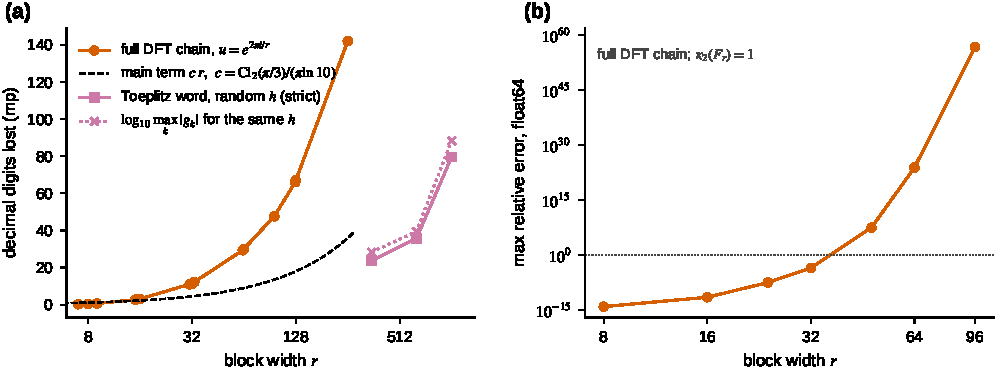
\includegraphics[width=\linewidth]{fig5_precision.pdf}
\caption{(a) Decimal digits lost in mp: full DFT chain (\cref{tab:mp}, all widths 7--256), Toeplitz word with random $h$ (\cref{tab:randtoep}) together with $\log_{10}\max_k\abs{g_k}$ for the same $h$, and the asymptotic leading term $cr$, $c=\Cl(\pi/3)/(\pi\ln10)$. (b) Relative error of the full chain in float64 (\cref{tab:float}); $\kappa_2(F_r)=1$.}\label{fig:precision}
\end{figure}

\begin{table}[tb]
\centering\small
\caption{Digit loss by stage (one random $x$). Local: the stage at working precision applied to the exact input; growth: $\log_{10}$ of the maximum modulus of an intermediate coordinate over the maximum modulus of the stage input.}\label{tab:stage}
\begin{tabular}{@{}rccccc@{}}
\toprule
$r$ & Stage & Local loss & Accumulated loss & Growth & $\log_{10}$ output norm \\
\midrule
\gentable{2b}
\bottomrule
\end{tabular}
\end{table}

\paragraph{Stage-wise loss (\cref{tab:stage,fig:stagewise}).}
(1)~The diagonal stages lose almost no digits ($\le2$); the whole loss falls on the two Toeplitz words. (2)~For $T^{\T}$ the local loss nearly equals the growth of intermediate values (5.6 and 6.5; 17.5 and 19.1; 42.4 and 43.9): the error behaves like $\varepsilon$ times the largest intermediate quantity. (3)~For $T$ the local loss exceeds the growth; it is comparable with $\log_{10}\kappa_2(T)$ plus the growth (at $r=64$: $9.0+9.2\approx18$ against 21.9), i.e.\ here the amplification of the input error by the operator itself is added. (4)~The total loss (\cref{tab:mp}) amounts to 2.5, 3.3, 3.7 and 4.0 units of $\log_{10}\kappa_2(T)$ at $r=32,64,128,256$.

\begin{figure}[t]
\centering
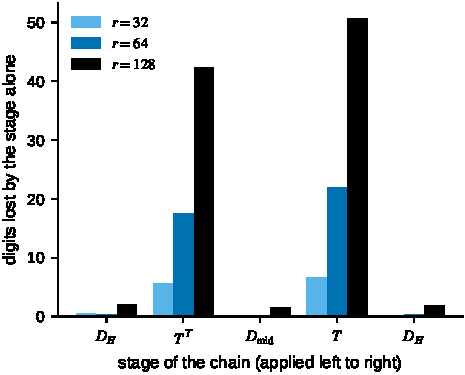
\includegraphics[width=0.55\linewidth]{fig6_stagewise.pdf}
\caption{Local digit loss by stage of the chain $\Dh$, $T^{\T}$, $\Dmid$, $T$, $\Dh$ at $r=32,64,128$ (\cref{tab:stage}).}\label{fig:stagewise}
\end{figure}

\paragraph{Where the growth arises (\cref{tab:growth} in \cref{app:tables}).}
The growth decomposition of \cref{sec:stagewise} describes growth, which can amplify rounding in $T^{\T}$ (where the local loss nearly equals the growth); for $T$ the loss exceeds the growth, so there the decomposition describes growth only. Its sums coincide with the growth column of \cref{tab:stage} ($T^{\T}$: 6.5, 19.1, 43.9; $T$: 3.0, 9.2, 21.7). (1)~All of the record-maximum growth of $T^{\T}$ occurs in the cross-block chunk phase, i.e.\ in the replay of displacement DAGs built from the reciprocal series $g$, not in leaf or direct layers. For $T$ the chunk phase gives 67--84\%, the rest the direct triangular word of base blocks of width 8 (below $v=10$ there is no admissible chunk, \cref{sec:counting}). (2)~The growth is distributed over several recursion levels rather than concentrated in one. In $T^{\T}$ the outer level $v=r$ contributes most (49--66\%); in $T$ the contribution shifts to middle levels. A zero increment at some level (for example $v=16$ for $T^{\T}$ at $r=128$) means only that no new record occurs there, not that the level does not contribute to the error. (3)~Hence the large intermediate quantities are localised in the displacement replay of chunks (growth of the reciprocal series $g$, \cref{sec:res-random}) and accumulate over recursion levels.

\paragraph{Phase-precision control (\cref{tab:phase} in \cref{app:tables}).}
Raising the precision of the chunk phase alone reduces the loss of $T^{\T}$ by about 14.5 and 37.5 digits at $r=64$ and $128$; raising the precision of the direct phase alone has almost no effect. For $T$ the reduction is about 10.3 and 27.9 digits, but a residual loss of 11.6 and 22.6 digits remains. Thus, for the checked inputs and widths, the precision of the chunks strongly affects the error of both stages, especially of $T^{\T}$. This is not an additive decomposition of the error: rounding in the phases and subsequent amplification interact, and the remainder cannot be called mere propagation without a separate control. The experiment covers one random vector (seed $=r$) per width, the fixed DFT coefficients, and $r=64,128$; it does not cover other coefficient distributions or wider cases.

\subsection{Toeplitz word with random coefficients}\label{sec:res-random}
This is a test of the general Toeplitz operator $Tx$, not of the DFT, run in strict mode with three vectors and two precisions (\cref{tab:randtoep}). For comparison, the zero-skipping variant with one vector lost 23.6, 35.0 and 78.6 digits at $r=352,640,1024$.

\begin{table}[tb]
\centering\small
\caption{Toeplitz word, random $h$, strict mode.}\label{tab:randtoep}
\begin{tabular}{@{}rcccc@{}}
\toprule
$r$ & Precision, digits & Max relative error & Digits lost & $\log_{10}\max_k\abs{g_k}$ \\
\midrule
\gentable{3}
\bottomrule
\end{tabular}
\end{table}

\paragraph{Mechanism of coefficient growth.}
The series $g$ is the reciprocal series of $h$ (\code{loc:reciprocal}) from which the chunks are built; its radius of convergence equals the smallest modulus $\rho$ of a root of $h(z)=\sum_k h_kz^k$. Hence $\log_{10}\abs{g_k}$ grows with slope $\log_{10}(1/\rho)$.

\begin{table}[tb]
\centering\small
\caption{Roots of $h(z)$ and growth of $g$ (\code{roots\_h.py}; roots are eigenvalues of the companion matrix, relative residual $\abs{h(z)}$ at the smallest roots $\le4\cdot10^{-14}$). The slope is fitted on the second half of $k$.}\label{tab:roots}
\begin{tabular}{@{}rcccccc@{}}
\toprule
$r$ & \hd{$\rho=\min\abs{\text{root}}$} & \hd{Roots inside\\unit disc} & \hd{Slope of\\$\log_{10}\abs{g_k}$} & $\log_{10}(1/\rho)$ & \hd{$(r-1)\log_{10}(1/\rho)$} & \hd{Observed\\$\log_{10}\max_{k<r}\abs{g_k}$} \\
\midrule
\gentable{3a}
\bottomrule
\end{tabular}
\end{table}

The slope coincides with $\log_{10}(1/\rho)$ to the fourth decimal, and the prediction $(r-1)\log_{10}(1/\rho)$ differs from the observed maximum by less than one digit (\cref{tab:roots}). About half of the roots lie inside the unit disc; the smallest modulus is 0.82--0.86. Thus, for these three samples, the growth of $g$ is explained by the smallest root of $h(z)$, and the digit loss nearly equals $\log_{10}\max_k\abs{g_k}$. We did not study the distribution of $\rho$ for other coefficient distributions.

\subsection{Fixed topology}\label{sec:res-topology}
For every run we compute SHA-256 of the sequence of layers, each layer recorded as its ASAP round and its list of gates (type M for scaling or S for shear, source, destination). The audit covers 12 widths, 2 rules (adaptive and chunk size 1) and 3 inputs (seed $=r$, another seed, $h=$ ones); the complete data are in \cref{tab:topology} (\cref{app:tables}). For every width and rule the hash is identical for all three inputs. Hence, in strict mode, the gate types, the coordinate pairs, the order of layers, the schedule by rounds, the depth and the gate count are functions of the width alone. Together with the static audit of \cref{sec:strict}, this confirms the fixed-topology requirement of the preprint for our implementation. For comparison, in the zero-skipping variant the depth at $r=64$ was 24442 and 24452 for two seeds and 13969 for $h=$ ones.

\subsection{Depth}\label{sec:res-depth}
The strict ASAP depth was measured on a grid of 12 widths: 64, 128, 256, 288, 320, 336, 352, 384, 512, 640, 768, 1024 (\code{strict\_tables.py}; data in \code{paper/data/strict\_tables.csv}).

\begin{table}[tb]
\centering\small
\caption{Strict ASAP depth: adaptive rule versus chunk size 1. The last column is the depth ratio of the value-dependent zero-skipping variant (archival data).}\label{tab:depth}
\begin{tabular}{@{}rcrrcc@{}}
\toprule
$r$ & $b$ & Adaptive & Chunk 1 & \hd{Adaptive /\\chunk 1} & \hd{Zero-skipping variant,\\adaptive / chunk 1} \\
\midrule
\gentable{5}
\bottomrule
\end{tabular}
\end{table}

In strict mode the adaptive rule has depth not larger than chunk size 1 at all 12 widths of the grid, and strictly smaller from $r=128$ on (\cref{tab:depth,fig:depth}). The crossover between 320 and 336 seen in the zero-skipping variant disappears: there chunk size 1 gained an advantage because in the DAGs for chunks of size 1 many pointwise multipliers are exactly zero ($g(1)=6$ instead of 8, $L(1)=18$ instead of 28). The jump of the ratio between 320 and 336 coincides with the jump of $b$ from 2 to 3 and persists in both modes. These conclusions concern this grid; we do not claim them for intermediate $r$. The depth is not monotone in $r$: at $r=352$ it is smaller than at $r=320$, because the larger block admits a larger chunk.

\begin{figure}[t]
\centering
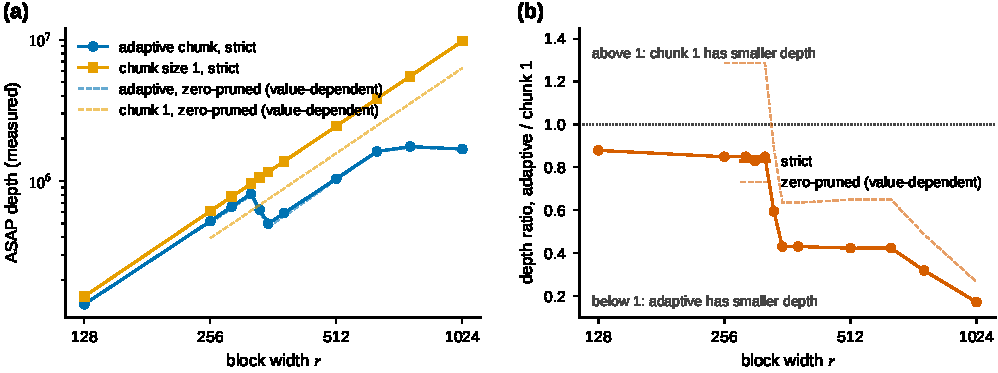
\includegraphics[width=\linewidth]{fig1_depth.pdf}
\caption{(a) Measured ASAP depth of the strict word for the adaptive rule and chunk size 1 (solid lines) and the same quantity for the value-dependent zero-pruned variant (thin dashed lines, archival data). Logarithmic axes. (b) Depth ratio adaptive / chunk 1; dotted line: equality. Below 1 the adaptive rule has smaller depth. In strict mode the ratio is below 1 at all widths from 128 on; the crossover of the zero-pruned variant near $r\approx330$ is an artifact of zero skipping. Data: \cref{tab:depth}.}\label{fig:depth}
\end{figure}

\paragraph{Depth model.}
We use the recurrence
\begin{equation}\label{eq:depth-model}
d(v)=d(\lfloor v/2\rfloor)+k^2L(b),\qquad k=\bigl\lceil\lfloor v/2\rfloor/b\bigr\rceil,
\end{equation}
with direct cost $v(v+1)/2$ for blocks without an admissible chunk; $b$ follows the strict table of $g(b)$, and $L(b)$ is the number of replay layers of one $b\times b$ pair in strict mode (\code{depth\_exact\_rule.py --strict}). The model uses the measured $g(b)$ and $L(b)$ and follows only the branch $\lfloor v/2\rfloor$; for powers of two both branches coincide.

\begin{table}[tb]
\centering\small
\begin{minipage}[t]{0.48\linewidth}\centering
\caption{Strict depth model versus measured ASAP depth (adaptive rule).}\label{tab:model}
\begin{tabular}{@{}rrrc@{}}
\toprule
$r$ & Model & ASAP & ASAP / model \\
\midrule
\gentable{6a}
\bottomrule
\end{tabular}
\end{minipage}\hfill
\begin{minipage}[t]{0.48\linewidth}\centering
\vspace{0pt}
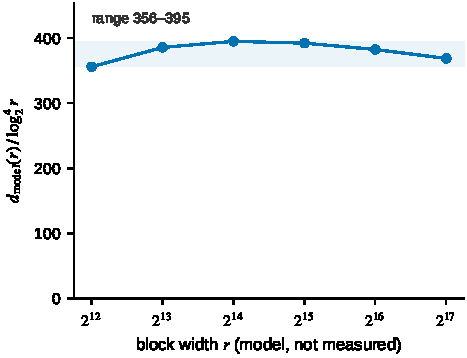
\includegraphics[width=\linewidth]{fig3_log4_law.pdf}
\captionof{figure}{Ratio $d_{\mathrm{model}}(r)/\log_2^4 r$ of the strict depth model at powers of two $2^{12}$--$2^{17}$; the band marks the range of values. Model values, not measurements. Data: \cref{tab:model-pow2}.}\label{fig:log4}
\end{minipage}
\end{table}

The model matches the measurement exactly at 10 of 12 widths (\cref{tab:model}). At $r=336$ and $352$ the recursion reaches odd blocks $v\ge10$ (21 and 11), and the model, which follows only the branch $\lfloor v/2\rfloor$, underestimates the depth. This directly confirms that the full recurrence must take the maximum over both branches, as in the preprint's proof \eqref{eq:depth-rec}.

At powers of two $2^{12}$--$2^{17}$ the model gives $d_{\mathrm{model}}/\log_2^4 r$ within 356--395 (\cref{tab:model-pow2} in \cref{app:tables}, \cref{fig:log4}). These values come from the model; we did not build ASAP words of these widths. Because the model is built on the empirical $g(b)$ and $L(b)$, its agreement with the measurements is a consistency check, not an independent proof of $O(\log^4 r)$. The order-of-magnitude heuristic
\begin{equation}\label{eq:heuristic}
g(b)\approx C\,b\log b\ \Rightarrow\ b=\Theta(v/\log v),\quad k=\Theta(\log v),\quad L(b)=\Theta(\log v),
\end{equation}
so that one level contributes $\Theta(\log^3 v)$ over $\log_2 r$ levels, explains why the model behaves like $\log^4 r$ and matches the preprint's proof of the upper bound. Six nearly constant points are consistent with $O(\log^4 r)$ but do not establish an asymptotic equality.

\subsection{Cost in identical units}\label{sec:res-cost}
\Cref{tab:flops} gives real flops (strict mode, adaptive rule, units of \cref{sec:cost-units}).

\begin{table}[tb]
\centering\footnotesize
\setlength{\tabcolsep}{2.5pt}
\caption{Real flops. Ratios are DFT via the word over radix-2 FFT, and one Toeplitz word over circulant-FFT and direct Toeplitz multiplication.}\label{tab:flops}
\begin{tabular}{@{}rrrrrrrrr@{}}
\toprule
$r$ & \hd{One Toeplitz\\word} & \hd{DFT via\\word} & \hd{Radix-2\\FFT} & \hd{Toeplitz via\\circulant FFT} & \hd{Direct\\Toeplitz} & \hd{DFT via word\\/ FFT} & \hd{Word /\\circulant FFT} & \hd{Word /\\direct} \\
\midrule
\gentable{7}
\bottomrule
\end{tabular}
\end{table}

The gate count of one word divided by $r^2$ is 15.8, 56.7, 77.1, 74.9 and 61.6 at $r=64,\dots,1024$. This quantity is not constant, so the data do not establish a quadratic cost law. At the checked widths the word is more expensive even than direct multiplication (\cref{fig:cost}). This is the cost of stand-alone execution of the word; the preprint does not use the word this way and claims no advantage at these widths (\cref{sec:cost-units}). The preprint cites Alman and Rao~\citep{alman2023} with leading term $(15/4)\,n\log_2 n$ real operations for the DFT at powers of two; against this reference the gap would be even larger.

\begin{figure}[t]
\centering
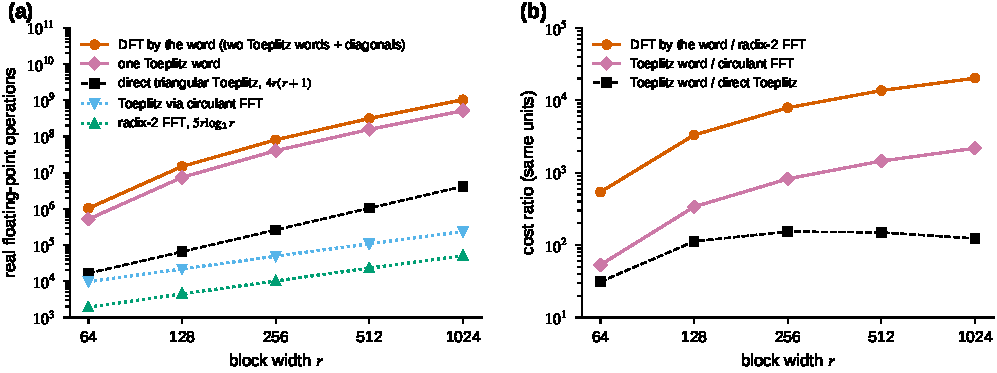
\includegraphics[width=\linewidth]{fig2_cost.pdf}
\caption{(a) Real flops of the DFT via the word, one Toeplitz word, direct Toeplitz multiplication, Toeplitz multiplication via circulant FFT, and radix-2 FFT. (b) Cost ratios in the same units. Data: \cref{tab:flops}.}\label{fig:cost}
\end{figure}

\paragraph{Gate--depth trade-off at $r=512$ (\cref{fig:tradeoff}).}
Strict mode, three rules:
\begin{itemize}
\item adaptive ($b=4$): depth 1\,035\,044, 19\,638\,528 gates;
\item chunk size 1: depth 2\,446\,116, 4\,647\,168 gates;
\item cap2 ($b\le2$): depth 2\,059\,044, 22\,882\,560 gates.
\end{itemize}
The adaptive rule and chunk size 1 form a trade-off: chunk size 1 has 4.2 times fewer gates and 2.4 times larger depth. cap2 is worse than the adaptive rule in both measures, i.e.\ it is dominated among these three rules. Only three rules were checked. Other chunk sizes, different rules at different recursion levels, or another schedule could give better points, so we do not claim that no rule minimises both quantities.

\begin{figure}[t]
\centering
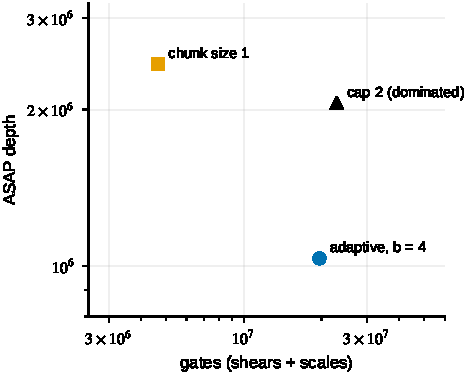
\includegraphics[width=0.5\linewidth]{fig4_tradeoff_r512.pdf}
\caption{Gates and depth at $r=512$ for three rules in strict mode. Both axes logarithmic. There is no spread over inputs, because the topology is fixed.}\label{fig:tradeoff}
\end{figure}

\subsection{Rounds and conflicts}\label{sec:res-rounds}
In strict mode (\code{rounds\_check.py}) execution by rounds gives the same result as sequential execution: the difference is 0.0 at $r=16,32,48,64$. Within a round there are no coordinate conflicts: 0 at $r=256$ (779\,392 layers, 518\,948 rounds, 1.50 layers per round) and at $r=512$ (2\,074\,880 layers, 1\,035\,044 rounds, 2.00 layers per round).

\subsection{Time and memory of our implementation}\label{sec:res-time}
One process per width, float64, strict mode, adaptive rule, the machine of \cref{sec:env}, command \code{timing.py r}. We measure one Toeplitz word on random complex $h$ and $x$ (\code{numpy.default\_rng(r)}, real and imaginary parts \code{standard\_normal}, $h_0$ replaced by $\abs{h_0}+1$), not the full DFT chain with two words and diagonal factors. The code labels RSS as GB, but \code{ru\_maxrss}$/1024^2$ on Linux gives GiB; the tables use GiB.

The measurement of \cref{tab:timing} was made on 2026-10-14 in the run \code{full-20261013-r3}. The run executes its steps sequentially, so the steps \code{timing-64}, \dots, \code{timing-512} did not overlap with other steps of the run; each is a separate process in a clean virtual environment (Python 3.12.3, numpy 1.26.4) with \code{OPENBLAS\_NUM\_THREADS} $=$ \code{OMP\_NUM\_THREADS} $=$ \code{MKL\_NUM\_THREADS} $=1$. Other processes on the machine were not controlled. The four steps together took 24~s. An earlier measurement with the same command, taken while seven other single-threaded computations (of 32 threads) ran on the machine, is kept unchanged as a record of those conditions in \cref{tab:timing-hist} (\cref{app:tables}).

\begin{table}[tb]
\centering\small
\caption{Python implementation (\code{timing.py}), measurement of 2026-10-14 without parallel steps of the run. Build: preparation of scalars and schedule.}\label{tab:timing}
\begin{tabular}{@{}rrccccc@{}}
\toprule
$r$ & Gates & \hd{Build of\\word, s} & \hd{Apply to one\\vector, s} & \hd{Peak\\memory, GiB} & \hd{numpy.fft of\\length $r$, \textmu s} & \hd{Dense Toeplitz\\product (numpy), \textmu s} \\
\midrule
\gentable{8a}
\bottomrule
\end{tabular}
\end{table}

In these timing runs the intermediate values overflow in float64 for $r\ge256$, so the outputs are not used as a correctness check; the time measures the execution of the same fixed gate list in Python, while exact correctness and numerical behaviour were checked by the separate experiments above. The gate counts are identical in both measurements and equal the sum of shears and scalings of the adaptive word in \cref{tab:topology}. The ratio of the repeat time to the earlier one is 0.81--0.88 for the build, 0.81--1.00 for the application and 0.73--0.81 for \code{numpy.fft}. Building the word in mp is more expensive: 7--83~s at $r=127$--256 with 250--450 digits in the earlier logs (\cref{tab:mp}) and 3--79~s in the repeat run. These numbers describe our Python implementation on this machine, not the algorithm of the preprint. They show the order of magnitude: our implementation applies one word roughly $10^4$ ($r=64$) to $10^6$ ($r=512$) times slower than \code{numpy.fft} performs the whole transform (both in the repeat and in the earlier measurement), and the memory grows with the gate count. At $r=512$ the word is built in 13.2~s (15~s in the earlier measurement).

% =====================================================================
\section{Discussion}\label{sec:discussion}

\subsection{The exponent and the full formula}\label{sec:disc-theta}
With $\delta$ from \eqref{eq:delta}, the ratio of the leading factors is
\begin{equation}\label{eq:ratio}
\frac{n(\log n)^{\theta}(\log\log n)^{4-\theta}}{n\log n}=\frac{(\log\log n)^{3+\delta}}{(\log n)^{\delta}} .
\end{equation}
It tends to zero, so the claimed bound is indeed $o(n\log n)$. At practical $n$, however, it is large. At $n=10^{300}$ with natural logarithms ($\ln n\approx690.8$, $\ln\ln n\approx6.54$) the ratio is $\approx279.446$, ignoring hidden constants (with $\log_2$ it would be $\approx988$). The ratio drops below 1 only when
\begin{equation}\label{eq:crossover}
\delta\,\ln\ln n>(3+\delta)\,\ln(\ln\ln n),\qquad\text{i.e.\ at }\ln\ln n\approx4.81494\cdot10^{14}.
\end{equation}
This is not a forecast of running time, but an explanation of why a small difference of exponents does not mean a practical speed-up. The numerical value of $\theta$ was recomputed in \cref{sec:constants}; our finite local experiments do not test the claimed global asymptotic time bound, which requires an analytical or formal proof.

\subsection{The scale gap}\label{sec:disc-scale}
$m=10^6$ and $W_*=2^{71}$ are parameters of the tensor network, not widths of the local compiler. The local widths in the proof are the first $\ell$ odd primes and one power of two $2^e<2r_{\ell+1}$, $\ell=\Theta(\log n/\log\log n)$ (\code{all-lengths.tex:13--56}); widths of these types (odd primes such as 7, 31 and 127, and powers of two) are partly covered by our tests. The concrete network recursion applies only in sectors with $k\ge K=m(71+1)=72\,000\,000$ axes (\code{network.tex:494--498}), and $k\le\ell$ (\code{synchronization.tex:82}). Then $\ell\ge72\,000\,000$, and already the elementary lower bound $r_\ell\ge\ell+2$ shows that the largest local width exceeds 1024 by a factor of more than 70 thousand. This compares the largest width; it does not claim that all axes are large. Extrapolating our numerical behaviour to these widths is not justified.

\subsection{Work versus time}
The preprint bounds the full time, including scalar preparation and index work. We count gates of the word and their flops, and measure time and memory only for our implementation (\cref{tab:timing,tab:timing-hist}).

\subsection{Value-dependent optimisations}\label{sec:disc-value}
Skipping zero multipliers does not change the operator, so it is admissible for a numerical implementation of the operator. But it lies outside the construction of the preprint, since it needs a zero test on a complex coefficient that the construction does not use (\code{local.tex:42}), and it changes the object being measured: depth and work become properties of the pair (width, coefficients) rather than of the width. The methodological lesson is direct: a value-dependent variant can produce structural effects that do not exist in the construction under test. In our case it produced a spurious depth crossover between $r=320$ and $336$ and a spurious seed-to-seed spread of the depth (\cref{sec:strict}); all results reported here use the strict construction. Degenerate inputs ($h=$ ones) are interesting in themselves and should be analysed separately rather than excluded; in strict mode they give the same structure as generic ones.

\subsection{Numerical instability}\label{sec:disc-instability}
The construction of the preprint is designed for exact arithmetic, and the preprint claims no stability. Our data show how much this restriction matters. In the Fourier case the conditioning of the Toeplitz factor grows roughly like $10^{cr}$ with $c=\Cl(\pi/3)/(\pi\ln10)\approx0.1403$ (the asymptotic leading term of the finite conditioning of $\Dh$), and the full chain loses 3--4 such units, i.e.\ about $0.5\,r$ decimal digits (142 at $r=256$). In float64 the chain is unusable already from $r\approx32$. The ordinary FFT is stable. Direct execution of this word (with the natural node order) in finite precision would require, at the checked widths, a number of digits growing roughly linearly with $r$; this changes the bit cost. The preprint does not claim anything about bit complexity (\code{introduction.tex:101}), so this is not a contradiction but a quantitative illustration of a limitation it names itself. The conclusion concerns only the local component: it does not mean that the full algorithm is unstable in every implementation, and it does not establish a lower bound on the cost of other modifications.

\subsection{Lower bounds}
The bounds of Morgenstern and Ailon concern bounded coefficients, unitary gates or bounded conditioning. Our data show that the local compiler indeed lies outside these frameworks: the conditioning of its factors grows exponentially with $r$. This is consistent with the bounds not applying to it, but says nothing about the correctness of the network.

\subsection{Implications for the preprint}\label{sec:implications}
Within the checked range the local component behaves as claimed: the implemented operator equals $F_r(u)$ (proved by computation in $\Q(\zeta_N)$ for eight widths 4--32; consistent with equality for the other checked $r$), the topology of the strict word depends only on $r$, and the depth model is compatible with $O(\log^4 r)$. We found no discrepancies with the claims of the preprint. This neither confirms nor refutes the main theorem, whose effect comes from the network. Checking the proof of the preprint itself requires an audit of the network and of the synchronisation; the comparison of the Lean definitions is complete within the scope of \cref{sec:lean}. Our measurements quantify, for the local component, limitations that the preprint names itself (enormous constants, exact arithmetic; \code{introduction.tex:67}, \code{:101}) and agree with the practical remarks of Recht~\citep{recht2026}; they say nothing about the correctness of the preprint.

% =====================================================================
\section{Limitations and threats to validity}\label{sec:limitations}

\paragraph{Scope of the checks.}
The full DFT is proved by computation in $\Q(\zeta_N)$ at eight widths from 4 to 32; in $\Fp$ (necessary condition) it is checked for the whole matrix at ten selected widths from 9 to 128, for a few vectors at $r=255,256,512$, and separately in streaming mode at $r=1024$ (the same two vectors in two fields); in mp at $r\le256$. The $C$-slots are proved by computation in $\Q(\zeta_N)$ at $r=4,8,16$, checked in $\Fp$ for the whole matrix at $r=16,31,32,33,64$ and by sampling at $r=128$, and in mp at $r\le256$. The Toeplitz word with random $h$ is checked at $r\le1024$; depth is measured at $r\le1024$ and modelled up to $r=2^{17}$. In mp at $r=96,127,256$ and in $\Fp$ at $r=255,256,512$ a few random vectors were checked rather than the whole matrix; in $\Fp$ at $r=127$ all basis vectors were checked.

\paragraph{Strength of evidence.}
Exact checks in $\Fp$ are a necessary condition, not a proof of the complex equality; only the checks in $\Q(\zeta_N)$ are proofs by computation. Agreement in mp is numerical agreement only.

\paragraph{Depth.}
The ASAP depth is a particular schedule, neither an optimum nor a lower bound. The equivalence of our chunk rule with the preprint's is established only for $b\le1024$ (\cref{sec:chunk}). The depth model uses the empirical $g(b)$ and $L(b)$ and follows only the branch $\lfloor v/2\rfloor$.

\paragraph{Instability analysis.}
Stage-wise measurements describe the observed distribution of digit loss (\cref{tab:stage}); the growth decomposition describes record-maximum increases over recursion levels and phases (\cref{tab:growth}); and the phase-precision control (\cref{tab:phase}, $r=64,128$) measures the sensitivity of the error to the precision of the cross-block chunks for the checked inputs. Together, these diagnostics do not provide a complete causal decomposition of rounding error. This control does not cover coefficient preparation, and for $T$ a significant loss remains after it. Not done: a decomposition down to individual chunks, a control for other coefficient distributions with possible cancellation, and widths beyond $r=128$.

\paragraph{Cost.}
Scalar preparation, indices and memory were measured only for our Python implementation; flops are counted by the standard scheme without special coefficients.

\paragraph{Lean.}
We rechecked the closure of the main goal, the axioms, and the correspondence of the definitions \code{DFTGoal}/\code{ConvGoal}/\code{RAM} with the statements of the preprint. The formalisation proves the required bound through a different network; \code{network.tex}, $\Delta$ and \code{net:tensor-bound} are not checked by it. We did not reread the proof bodies; the correspondence of \code{Bill} with a physical word-RAM remains a modelling judgement; there is no separate simulation theorem. This is a reproduction of someone else's mechanical check, not our own independent proof.

\paragraph{Main theorem.}
The numerical value of $\theta$ was recomputed (\cref{sec:constants}), but the main asymptotic saving, the network, the synchronisation, the algorithm for lengths of all sizes and the synthesis were not checked by local experiments.

\paragraph{Threats to validity.}
The exact checks are executed by \code{generic\_word.py}, whereas the numerical ones use \code{mp\_exact}/\code{mp\_compiler} and \code{conv\_dag}/\code{rounds}. These are separate implementations of one described construction, so equality in an exact field applies directly to the exact checker. An additional comparison of the sequences of layers and coordinate pairs (without coefficients) showed that the three strict builders coincide at $r=4,7,8,9,12,15,16,31,32,33,64,128$ for $h_k=1/(k+1)$; this supports structural correspondence but is not a proof that their coefficients coincide, nor a statement for all widths. Our own shear decomposition, the early stopping of the chunk rule and the ASAP schedule are implementation choices; their checked limits are stated above. The phase and random-Toeplitz diagnostics use one seed per width; no broader statistical generalisation is claimed. Timings depend on the machine and on concurrent load.

% =====================================================================
\section{Data and code availability}\label{sec:availability}
The code, the data, and the raw logs of the complete run \code{full-20261013-r3}, together with its manifest and hashes, will be available at \url{https://github.com/cyberdid/fft-power-saving-verification} under the Apache License 2.0. Paths below are relative to the root of that repository.

\begin{itemize}
\item \code{release/README\_REPRODUCE.md}: reproduction steps and the mapping from scripts to tables.
\item \code{release/run\_all.sh quick|full}: an isolated run, i.e.\ a copy of the sources, then raw results, then the CSV files of this run, then validation of all tables of the manuscript against them, then the figures from the same CSV files. Every run has its own directory and a manifest of commands, exit codes and hashes. Mode \code{full} executes all 135 steps; mode \code{quick} explicitly skips the six longest experiments and therefore does not confirm a full reproduction. An interrupted run can be resumed in the same environment; resumption checks that the captured sources, the environment and the results of completed steps are unchanged.
\item \code{release/evidence/full-20261013-r3/}: the raw logs, aggregated data, figures, environment freeze and manifest of the complete run used in this paper; the manifest records the SHA-256 of every captured source file, of every log and of every output. The files are byte-identical to those of the run and therefore keep the absolute paths of the machine on which it was executed. The comparison curves of the zero-pruned variant in \cref{fig:depth} are archival and labelled as such.
\item \code{paper/data/supplemental/fp1024/}: data, logs and reproduction instructions of the separate streaming $\Fp$ test at $r=1024$ (\code{paper/scripts/stream\_exact\_dft.py}), which is not one of the 135 steps.
\item \code{release/requirements-lock.txt}: pinned direct and transitive dependencies, installed into a clean environment with a successful \code{pip check}; \code{release/requirements-full-freeze.txt}: the full freeze of the development environment (a record, not a lock file); \code{release/ENVIRONMENT.txt}.
\item \code{release/lean/}: \code{lean-toolchain}, \code{lakefile.lean}, \code{lake-manifest.json}, \code{AxiomCheck.lean}, \code{MODEL\_AUDIT.md} and the build logs.
\item \code{release/SHA256SUMS}: checksums of the code, data and figures of this version; it certifies the integrity of the recorded files, not the proof of any theorem.
\end{itemize}
The code is in \code{allength/} (among others \code{conv\_dag.py} with the flag \code{KEEP\_ZERO\_MULTIPLIERS}, \code{mp\_exact.py} with \code{ROOT\_SIGN}, \code{exact\_field.py}, \code{generic\_word.py}, \code{rounds.py}, \code{mp\_compiler.py}, \code{compiler.py}, \code{depth\_recurrence.py}); scripts are in \code{paper/scripts/}, aggregated data in \code{paper/data/*.csv}. The preprint is available in the repository \url{https://github.com/openai/math} (directory commit 301488868, HEAD fd4aeeb).

% =====================================================================
\section{Conclusion}\label{sec:conclusion}
We independently checked the local compiler of OpenAI's preprint in its strict form, in which the topology depends only on the width, and confirmed this property by a code audit and by structure hashes. For eight widths from 4 to 32 we proved by computation in cyclotomic fields that the matrix of the exact builder equals $F_r(u)$. For selected widths up to $r=512$, and in a separate streaming test at $r=1024$, exact checks in finite fields give a necessary condition (by sampling at $r=255,256,512,1024$), and high-precision arithmetic up to $r=256$ agrees with equality. The $C$-slot path (our shear decomposition; the splitting and the conjugation via the DAG with inverse roots as in the preprint) is proved by computation at $r=4,8,16$.

In finite precision this exact construction is strongly unstable; the preprint does not claim stability, so this contradicts none of its statements. The conditioning of the Toeplitz factor in the Fourier case grows roughly like $10^{cr}$, $c\approx0.1403$ (the asymptotic leading term of the finite conditioning, through the Clausen function); the full chain loses about $0.5\,r$ decimal digits, almost all of them in the two Toeplitz words, and is unusable in float64 already from $r\approx32$, although $\kappa_2(F_r)=1$. The measured depth of the strict word up to $r=1024$ and the depth model up to $2^{17}$ are compatible with the upper bound $O(\log^4 r)$. The cost of stand-alone execution of the word in real flops is two to four orders of magnitude above the FFT at the checked widths, and above even direct multiplication; the preprint does not use the word in this way (\cref{sec:cost-units}). A variant that drops exactly-zero multipliers is value-dependent and produces depth effects absent from the strict construction, which is why all results here use the latter.

Our local experiments do not test the main asymptotic saving with $\theta$. The Lean formalisation of OpenAI that we recompiled proves \code{DFTGoal} with the required upper bound through a different network; the concrete \code{network.tex} and its $\Delta$ are not checked by it. The comparison of definitions is complete within the scope of \cref{sec:lean}; the adequacy of \code{Bill} with respect to a physical RAM remains a modelling judgement, and we did not reread the proof bodies line by line. Our results neither refute the theorem nor constitute an independent proof of its main effect; they delimit the checked local implementation and the limits of its use in finite precision.

% =====================================================================
{\raggedright
\bibliographystyle{plainnat}
\bibliography{../refs}
\par}

% =====================================================================
\appendix

\section{Additional tables}\label{app:tables}

\begin{table}[tb]
\centering\small
\caption{Decomposition of the growth of intermediate quantities by levels and phases (one random $x$, seed $=r$; growth in $\log_{10}$). The last column lists the increments by block width $v$.}\label{tab:growth}
\begin{tabularx}{\linewidth}{@{}rcccc L@{}}
\toprule
$r$ & Stage & Growth & \hd{In chunk\\phase} & \hd{In direct\\word} & Distribution over levels $v$ (increment) \\
\midrule
\gentable{2c}
\bottomrule
\end{tabularx}
\end{table}

\begin{table}[tb]
\centering\small
\caption{Digits lost at DPS when the selected phase is executed at reference precision and the rest at DPS; in parentheses the change relative to ``all at DPS''.}\label{tab:phase}
\begin{tabular}{@{}rccccc@{}}
\toprule
$r$ & Stage & DPS & All at DPS & \hd{Reference\\chunk phase} & \hd{Reference\\direct phase} \\
\midrule
\gentable{2d}
\bottomrule
\end{tabular}
\end{table}

\begin{table}[tb]
\centering\small
\begin{minipage}[t]{0.48\linewidth}\centering
\caption{Strict depth model at powers of two (model values, not measurements).}\label{tab:model-pow2}
\begin{tabular}{@{}rrrc@{}}
\toprule
$r$ & $b$ & $d_{\mathrm{model}}(r)$ & $d_{\mathrm{model}}/\log_2^4 r$ \\
\midrule
\gentable{6b}
\bottomrule
\end{tabular}
\end{minipage}\hfill
\begin{minipage}[t]{0.48\linewidth}\centering
\caption{Earlier timing measurement (\code{timing.py}), taken while seven other single-threaded computations ran on the machine. Columns as in \cref{tab:timing}.}\label{tab:timing-hist}
\setlength{\tabcolsep}{2.5pt}
\begin{tabular}{@{}rrccccc@{}}
\toprule
$r$ & Gates & \hd{Build,\\s} & \hd{Apply,\\s} & \hd{Mem.,\\GiB} & \hd{fft,\\\textmu s} & \hd{Dense,\\\textmu s} \\
\midrule
\gentable{8}
\bottomrule
\end{tabular}
\end{minipage}
\end{table}

\begin{table}[tb]
\centering\small
\caption{Topology audit of the strict word: 12 widths $\times$ 2 rules $\times$ 3 inputs (seed $=r$, another seed, $h=$ ones). The last column states whether the structure hash is identical for the three inputs.}\label{tab:topology}
\begin{tabular}{@{}rlrrrl@{}}
\toprule
$r$ & Rule & Depth & Layers & Gates & Identical hash \\
\midrule
\gentable{4}
\bottomrule
\end{tabular}
\end{table}

\clearpage
\section{Proofs and derivations}\label{app:proofs}

\subsection{Nonvanishing of the split coefficients}\label{app:kappa}
\begin{proof}[Proof of \cref{lem:split}]
Since $\kappa=1+\abs{\mu}^2$ is real and $\kappa\ge1$, we have $t_1=\kappa\ne0$. By the reverse triangle inequality, $\abs{t_2}=\abs{\kappa-\mu}\ge\abs{\kappa}-\abs{\mu}=1+\abs{\mu}^2-\abs{\mu}$. Completing the square,
\[
1+\abs{\mu}^2-\abs{\mu}=\Bigl(\abs{\mu}-\tfrac12\Bigr)^2+\tfrac34\ \ge\ \tfrac34>0 .
\]
Hence $t_2\ne0$, and $t_1+t_2=\mu$ for every $\mu$, including $\mu=0$. The argument uses that $\mu\bar\mu=\abs{\mu}^2$ is a nonnegative real number; it therefore does not transfer to $\Fp$, where the nonvanishing of $t_1,t_2$ is instead checked at each inversion (\cref{sec:exact}).
\end{proof}

\subsection{Clausen asymptotics of \texorpdfstring{$\log_{10}\kappa_2(D_H)$}{log10 kappa2(DH)}}\label{app:clausen}
Recall $\Cl(\varphi)=-\int_0^{\varphi}\log\abs{2\sin(t/2)}\,dt$; its maximum on $[0,2\pi]$ is at $\varphi=\pi/3$, $\Cl(\pi/3)\approx1.01494$, and $\Cl(2\pi-\varphi)=-\Cl(\varphi)$.
\begin{proposition}\label{prop:clausen}
For $u=e^{2\pi i/r}$ and $\Dh=\diag(H_0,\dots,H_{r-1})$,
\[
\log_{10}\kappa_2(\Dh)=\frac{r}{\pi}\,\frac{\Cl(\pi/3)}{\ln10}+o(r)\qquad(r\to\infty).
\]
\end{proposition}
\begin{proof}
For a diagonal matrix $\kappa_2(\Dh)=\max_k\abs{H_k}/\min_k\abs{H_k}$. Since $\abs{1-e^{2\pi is/r}}=2\sin(\pi s/r)$ for $0<s<r$,
\[
\ln\abs{H_k}=\sum_{s=1}^{k}\ln\bigl(2\sin(\pi s/r)\bigr).
\]
The summand is negative for $\pi s/r<\pi/6$ and for $\pi s/r>5\pi/6$ and positive in between; hence $\ln\abs{H_k}$ is minimal at $k\approx r/6$ and maximal at $k\approx5r/6$. Approximating the sum by an integral (the integrand has only integrable logarithmic singularities at the endpoints, so the error of the Riemann sum is $o(r)$) and substituting $t=x/2$,
\[
\ln\abs{H_k}=\frac{r}{\pi}\int_0^{\pi k/r}\ln(2\sin t)\,dt+o(r)=-\frac{r}{2\pi}\,\Cl\Bigl(\frac{2\pi k}{r}\Bigr)+o(r),
\]
uniformly in $k$. At $2\pi k/r=5\pi/3$ the value is $-\frac{r}{2\pi}\Cl(5\pi/3)=\frac{r}{2\pi}\Cl(\pi/3)$, and at $2\pi k/r=\pi/3$ it is $-\frac{r}{2\pi}\Cl(\pi/3)$. The difference is $\frac{r}{\pi}\Cl(\pi/3)+o(r)$; dividing by $\ln10$ gives the claim, with $c=\Cl(\pi/3)/(\pi\ln10)=0.14030576$.
\end{proof}
The finite values in \cref{tab:cond} are exact differences of partial sums; they differ from $cr$ by $o(r)$, e.g.\ by $10^{-4}$ at $r=1024$.

\subsection{Localisation for \texorpdfstring{$\mathbb{F}_p$}{Fp}}\label{app:localisation}
\begin{proof}[Proof of \cref{prop:localisation}]
Let $p=kN+1$ be prime and $\omega\in\Fp$ of multiplicative order $N$. Since $p\nmid N$, $\omega$ is a root of $\Phi_N$ modulo $p$, and $\zeta_N\mapsto\omega$ defines a surjective ring homomorphism $\phi:\Z[\zeta_N]\cong\Z[x]/(\Phi_N)\to\Fp$ with kernel $\mathfrak p$, a prime ideal. Let $R=\Z[\zeta_N]_{\mathfrak p}\subset\Q(\zeta_N)$ be the localisation, i.e.\ the fractions $a/b$ with $a,b\in\Z[\zeta_N]$ and $b\notin\mathfrak p$. Then $\phi$ extends uniquely to a ring homomorphism $\phi:R\to\Fp$, $\phi(a/b)=\phi(a)\phi(b)^{-1}$; rational constants with denominators prime to $p$ lie in $R$.

We show by induction along the straight-line program that every intermediate value $z$ lies in $R$ and that the value computed in $\Fp$ is $\phi(z)$. Inputs and constants satisfy this. Ring operations preserve $R$ and commute with $\phi$. If $z\in R$ is inverted and the $\Fp$ computation inverts $\phi(z)\ne0$, then $z\notin\mathfrak pR$, so $z$ is a unit of the local ring $R$, $z^{-1}\in R$ and $\phi(z^{-1})=\phi(z)^{-1}$. Thus the $\Fp$ output is the image of the $\Q(\zeta_N)$ output. If the latter equals $F_r(\zeta_r)$, the former equals $F_r(\phi(\zeta_r))$; contrapositively, a mismatch in $\Fp$ implies a mismatch over $\Q(\zeta_N)$, whereas agreement in $\Fp$ does not exclude a nonzero difference lying in $\mathfrak pR$.

Complex conjugation on $\Q(\zeta_N)$ is the automorphism $\sigma:\zeta_N\mapsto\zeta_N^{-1}$. The DAG evaluated with inverse roots computes $\sigma(\mu)=\bar\mu$ over $\Q(\zeta_N)$, and the same DAG evaluated in $\Fp$ with $\omega^{-1}$ in place of $\omega$ computes $\phi(\sigma(\mu))$ by the argument above. Hence the $\Fp$ check of the $C$-slot path tests the image of the same conjugate expression, although $\Fp$ itself has no nontrivial automorphism.
\end{proof}

\section{Summary of the Lean statement audit}\label{app:lean}
\Cref{tab:lean} summarises the comparison of the Lean definitions with the preprint (\cref{sec:lean}). Proof bodies were not reread; their correctness for these definitions is checked by the Lean kernel.

\begin{table}[tb]
\centering\small
\caption{Lean definitions versus the preprint. $G$ = \code{Goal.lean}, $R$ = \code{RAM.lean}, $C$ = \code{FourierCircuit/Core.lean}.}\label{tab:lean}
\begin{tabularx}{\linewidth}{@{}P{0.27\linewidth}LP{0.25\linewidth}@{}}
\toprule
Lean definition (file) & Content & Verdict \\
\midrule
\code{zeta}, \code{fourierMatrix} ($C$); \code{dft} ($G$) & $\zeta_n=\exp(2\pi i/n)$; $(\zeta_n^{jk})$; unnormalised $F_nx$ & Matches \code{introduction.tex} \\
Constants $m$, $W_*$, $\Delta$, $\lambda$, $\theta$ ($G$) & Same exact constants as \eqref{eq:constants} & Matches \\
\code{paperTime}, \code{decimalTime} ($G$) & $n(\ln n)^{\theta}(\ln\ln n)^{4-\theta}$; exponent $1-10^{-13}$; natural logarithms & Matches \code{thm:main}, \code{cor:decimal} \\
\code{DFTProgram} ($G$) & For all $n>0$: root order $0<D<1024\,n^3$ computed and charged in the model; $\code{d.work}+1+\code{result.work}\le W(n)$; result $=\code{dft}\,n\,x$ for all $x$ & Matches; root order is computed in the model (stronger) \\
\code{TimeBounds}, \code{DFTGoal} ($G$) & $W=O(\code{paperTime})$, $W=O(\code{decimalTime})$, $W=o(n\log n)$; fixed \code{order}, \code{solve}, $W$ & Matches \\
\code{ConvGoal} ($G$) & Bilinear products allowed (\code{Prog true}); result is the linear convolution & Matches; stronger (root bound, bilinear products only) \\
\code{Paint}, \code{Bill}, atoms ($R$) & Separate scalar and data registers; every atom costs 1; \code{inv} only on scalars with nonzero condition; no complex constants or $\C\leftrightarrow\mathbb N$ atoms; branching on integers only & Matches; no simulation theorem for word-RAM \\
\code{receipt} & $D=\code{receipt}(n)<8\,n^3$ in the \code{\_order} variants & Formula differs from $D_*$ (\code{eq:master-root}); bound satisfied \\
Internal network (\code{lunch\_big}, \code{alpha\_theta}) & 32 binary coordinates per factor, 4060 triples, bound $2^{50}$; $W=O\bigl(n(\ln n)^{\alpha}(\ln\ln n)^2\bigr)$, $\alpha=1-2\cdot10^{-11}<\theta$ & Different from \code{network.tex}; $\Delta$ and \code{net:tensor-bound} not checked \\
Axioms (all four main theorems) & \code{propext}, \code{Classical.choice}, \code{Quot.sound} & No \code{sorry}; 89 modules in the import closure \\
\bottomrule
\end{tabularx}
\end{table}

\end{document}
